\chapter{Dictionaries}
\label{chap-dictionaries}

\section{The DELA dictionaries}
\index{DELA}\index{Dictionaries!format}\index{LADL}

The electronic dictionaries distributed with Unitex use the DELA syntax
(Dictionnaires Electroniques du LADL, LADL electronic dictionaries). This syntax
describes the simple and compound lexical entries \index{Lexical!entries} of a
language with their grammatical, semantic and inflectional information. We
distinguish two kinds of electronic dictionaries. The one that is used most often
is the  dictionary of inflected forms DELAF (DELA de formes Fl\'echies, DELA of
inflected forms) or DELACF (DELA de formes Compos\'ees Fl\'echies, DELA of
compound inflected forms) in the case of compound forms.\index{DELAF|(}
\index{DELACF}\index{Dictionaries!DELAF|(}\index{Dictionaries!DELACF}
The second type is a dictionary of non-inflected forms called DELAS (DELA de
formes simples, simple forms DELA) or DELAC (DELA de formes compos\'ees,
compound forms DELA).
\index{DELAS}\index{DELAC}\index{Dictionaries!DELAS}\index{Dictionaries!DELAC}

\bigskip
\noindent Unitex programs make no  distinction between simple and compound form
dictionaries. We will use the terms DELAF and DELAS to distinguish the
inflected and non-inflected dictionaries, no matter they contain simple word,
compound words or both. 

\subsection{The DELAF format}
\label{section-DELAF-format}
\subsubsection{Entry syntax}
\label{section-DELAF-entry-syntax}
An entry of a DELAF is a line of text terminated by a newline that conforms to
the following syntax:

\bigskip
\begin{verbatim}
apples,apple.N+conc:p/this is an example
\end{verbatim}

\bigskip
\noindent The different elements of this line are:

\bigskip
\begin{itemize}
  \item \verb+apples+ is the inflected form of the entry;\index{Form!inflected} it is mandatory;
  
  \bigskip \item \verb+apple+ is the canonical form (lemma) of the
  entry.\index{Lemma} \index{Form!canonical}For nouns and adjectives (in French), it is usually the
  masculine singular form; for verbs, it is the infinitive. This information may
  be left out as in the following example:
  
  \bigskip
  \verb$apple,.N+Conc:s$
  
  \bigskip This means that the canonical form is the same as the inflected form.
  The canonical form is separated from the inflected form by a
  comma.\index{\verbc{,}}
  
  \bigskip \item \verb$N+Conc$ is the sequence of grammatical and semantic
  information. \index{Information!grammatical} \index{Information!semantic}In our
  example, \verb+N+ designates a noun, and \verb+Conc+ indicates that this noun
  designates a concrete object (see table~\ref{tab-semantic-codes}).
  
  Each entry must have at least one grammatical or semantic code, separated from
  the canonical form by a period. If there are more codes, these are separated by
  the \verb$+$\index{\verbc{+}}\index{\verbc{.}} character.
  
  \bigskip \item \verb+:p+ is an inflectional code which indicates that the noun
  is  plural.\index{Information!inflectional} Inflectional codes are used to
  describe gender, number, declension, and conjugation. This information is
  optional. An inflectional code is made up of one or more characters that
  represent one information each. Inflectional codes have to be separated by the
  "\verb+:+'' character, for instance in an entry like the following:
  
  \verb+hang,.V:W:P1s:P2s:P1p:P2p:P3p+
  
  The \verb+:+ character is interpreted in OR semantics. Thus,
  \verb+:W:P1s:P2s:P1p:P2p:P3p+ means "infinitive", or "1st person singular
  present", or "2nd person singular present", etc. (see
  table~\ref{tab-inflectional-codes}) Since each character
  represents one information, you must not use the same character
  more than once. In this way, encoding the past participle using the code \verb+:PP+ would be
  exactly equivalent to using \verb+:P+ alone;\index{\verbc{:}}
  
  \bigskip \item \verb+/this is an example+ is a comment. Comments are optional
  and are introduced by the \verb+/+ character. These comments are left out when
  the dictionaries are compressed. \index{Comment!in a dictionary}
  \index{Dictionaries!comments in} \index{\verbc{/}}
\end{itemize}

\bigskip
\noindent IMPORTANT REMARK: It is possible to use the full stop and the comma
within a dictionary entry. In order to do this they have to be escaped using the
\verb+\+ \index{\verbt{\textbackslash,}}\index{\verbt{\textbackslash.}}\index{\verbt{\textbackslash~}} character:

\bigskip
\begin{verbatim}
1\,000,one thousand.NUMBER
United Nations,U\.N\..ACRONYM
\end{verbatim}


\bigskip
\noindent WARNING: Each character is taken into account within a dictionary
line. For example, if you insert spaces, they are considered to be a part of the
information. In the following line:

\begin{verbatim}
hath,have.V:P3s /old form of 'has'
\end{verbatim}

\bigskip \noindent The space that precedes the \verb+/+ character will be
considered to be part of a 4-character inflectional code.

\bigskip \noindent It is possible to insert comments into a DELAF or DELAS
dictionary by starting the line with a $/$ character. Example:

\bigskip
\begin{verbatim}
/ 'English' designates a pool spin
English,.N+z3:s
\end{verbatim}


\subsubsection{Compound words with spaces or dashes}

\index{Words!compound!with space or dash}\index{\verbc{=}}\index{\verbt{\textbackslash=}}

Certain compound words like \textit{acorn-shell} can be written using spaces or
dashes. In order to avoid duplicating the entries, it is possible to use the
\verb+=+ character. At the time when the dictionary is compressed, the
\verb+Compress+ program \index{External
programs!\verbc{Compress}}\index{\verbc{Compress}} checks for each line if the
inflected or canonical form contains a non-escaped \verb+=+ character. If this is
the case, the program replaces this by two entries: one where the \verb+=+
character is replaced by a space, and one where it is replaced by a dash. Thus,
the following entry:

\bigskip \verb$acorn=shells,acorn=shell.N:p$

\bigskip
\noindent is replaced by the following entries:

\bigskip
\verb$acorn shells,acorn shell.N:p$

\verb$acorn-shells,acorn-shell.N:p$

\bigskip
\noindent NOTE: If you want to keep an entry that includes the \verb+=+
character, escape it using \verb+\+ as in the following example:

\bigskip \verb$E\=mc2,.FORMULA$

\bigskip
\noindent This replacement is done when the dictionary is compressed. In the compressed
dictionary, the escaped \verb+=+ characters are replaced by simple \verb+=+. As
such, if a dictionary containing the following lines is compressed:


\bigskip
\verb$E\=mc2,.FORMULA$

\bigskip
\verb$acorn=shell,.N:s$

\bigskip
\noindent and if the dictionary is applied to the following text:

\bigskip
\textit{Formulas like E=mc2 have nothing to do with acorn-shells.}

\bigskip \noindent you will get the following lines in the dictionary of compound
words of the text:


\begin{verbatim}
E=mc2,.FORMULA

acorn-shells,.N:p
\end{verbatim}


\subsubsection{Entry Factorization}

Several entries containing the same inflected and canonical forms can be
combined into a single one if they also share the same grammatical and semantic
codes. Among other things this allows us to combine identical conjugations for a verb:

\bigskip
\begin{verbatim}
bottle,.V:W:P1s:P2s:P1p:P2p:P3p
\end{verbatim}

\bigskip 
\noindent If the grammatical and semantic information differ, one has to create
distinct entries:

\bigskip
\begin{verbatim}
bottle,.N+Conc:s
bottle,.V:W:P1s:P2s:P1p:P2p:P3p
\end{verbatim}

\bigskip 
\noindent Some entries that have the same grammatical and semantic entries can
have different meanings, as it is the case for the French word \textit{po\^ele}
that describes a stove or a type of sheet in the masculine sense and a kitchen
instrument in the feminine sense. You can thus distinguish the entries in  this
case:

\bigskip
\noindent
\texttt{po\^ele,.N+z1:fs/ po\^ele \`a frire}

\noindent
\texttt{po\^ele,.N+z1:ms/ voile, linceul; appareil de chauffage}

\bigskip 
\noindent NOTE: In practice, this distinction has the only consequence that the
number of entries in the dictionary increases.

\bigskip 
\noindent For the different programs that make up Unitex these entries are equivalent to:

\bigskip
\noindent
\texttt{po\^ele,.N+z1:fs:ms}

\bigskip 
\noindent Whether this distinction is made is thus left to the  maintainers of  the dictionaries.

\index{DELAF|)}\index{Dictionaries!DELAF|)}

\subsection{The DELAS Format}
\label{section-DELAS-format}
\index{DELAS}\index{Dictionaries!DELAS}

The DELAS format is very similar to the one used in the DELAF. The only
difference is that there is only a canonical form followed by grammatical
and/or semantic codes. The canonical form is separated from the different codes
by a comma. There is an example: \index{\verbc{,}}

\begin{verbatim}
horse,N4+Anl
\end{verbatim}

\noindent The first grammatical or semantic code will be interpreted by the
inflection program as the name of the grammar used to inflect the entry. The entry of the
example above indicates that the word \textit{horse} has to be inflected using
the grammar named \verb+N4+. It is possible to add inflectional codes to the
entries, but the nature of the inflection operation limits the usefulness of this
possibility. For more details see below in
section~\ref{section-automatic-inflection}.


\subsection{Dictionary Contents}
\index{Dictionaries!contents}\index{Dictionaries!codes used within}

The dictionaries provided with Unitex contain descriptions of simple and compound
words. These descriptions indicate the grammatical category of each entry,
optionally their inflectional codes, and various semantic information. The
following tables give an overview of some of the different codes used in the 
Unitex dictionaries. These codes are the same for almost all languages, though
some of them are special for certain languages (\textit{i.e.} code for neuter
nouns, etc.).

\begin{table}[!ht]
\index{\verbc{A}}\index{\verbc{ADV}}\index{\verbc{CONJC}}\index{\verbc{CONJS}}\index{\verbc{DET}}
\index{\verbc{INTJ}}\index{\verbc{N}}\index{\verbc{PREP}}\index{\verbc{PRO}}\index{\verbc{V}}
\begin{center}
\begin{tabular}{|c|l|l|}
\hline
\textbf{Code} & \textbf{Description} & \textbf{Examples} \\
\hline
\verb+A+ & adjective & fabulous, broken-down \\
\hline
\verb+ADV+ & adverb & actually, years ago \\
\hline
\verb+CONJC+ & coordinating conjunction & but\\
\hline
\verb+CONJS+ & subordinating conjunction & because \\
\hline
\verb+DET+ & determiner & each \\
\hline
\verb+INTJ+ & interjection & eureka \\
\hline
\verb+N+ & noun & evidence, group theory \\
\hline
\verb+PREP+ & preposition & without \\
\hline
\verb+PRO+ & pronoun & you \\
\hline
\verb+V+ & verb & overeat, plug-and-play \\
\hline
\end{tabular}
\caption{Frequent grammatical codes\label{tab-grammatical-codes}}
\end{center}
\end{table}

\begin{table}[!ht]
\index{\verbc{z1}}\index{\verbc{z2}}\index{\verbc{z3}}\index{\verbc{Abst}}\index{\verbc{Anl}}\index{\verbc{AnlColl}}
\index{\verbc{Conc}}\index{\verbc{ConcColl}}\index{\verbc{Hum}}\index{\verbc{HumColl}}\index{\verbc{t}}\index{\verbc{i}}
\index{\verbc{en}}\index{\verbc{se}}\index{\verbc{ne}}
\begin{center}
\begin{tabular}{|c|l|l|}
\hline
\textbf{Code} & \textbf{Description} & \textbf{Example} \\
\hline
\verb+z1+ & general language & joke \\
\hline
\verb+z2+ & specialized language & floppy disk \\
\hline
\verb+z3+ & very specialized language & serialization \\
\hline
\verb+Abst+ & abstract & patricide \\
\hline
\verb+Anl+ & animal & horse \\
\hline
\verb+AnlColl+ & collective animal & flock \\
\hline
\verb+Conc+ & concrete & chair \\
\hline
\verb+ConcColl+ & collective concrete & rubble \\
\hline
\verb+Hum+ & human & teacher \\
\hline
\verb+HumColl+ & collective human & parliament \\
\hline
\verb+t+ & transitive verb & kill \\
\hline
\verb+i+ & intransitive verb & agree \\
\hline
\end{tabular}
\caption{Some semantic codes\label{tab-semantic-codes}}
\end{center}
\end{table}

\bigskip
\noindent NOTE: The  descriptions of tense in
table~\ref{tab-inflectional-codes} correspond to French.
Nontheless, the majority of these definitions can be found in other languages (infinitive, present, past participle, etc.).

\bigskip
\noindent In spite of a common base in the majority of languages, the dictionaries
contain encoding particularities that are specific for each language. Thus, as
inflectional codes vary a lot between different languages, they are not
described here. For a complete description of all codes used within a dictionary,
we recommend that you  contact the author of the dictionary directly.

\begin{table}[!ht]
\index{\verbc{m}}\index{\verbc{f}}\index{\verbc{n}}\index{\verbc{s}}\index{\verbc{p}}\index{\verbc{1}}
\index{\verbc{2}}\index{\verbc{3}}\index{\verbc{P}}\index{\verbc{I}}\index{\verbc{S}}\index{\verbc{T}}
\index{\verbc{Y}}\index{\verbc{C}}\index{\verbc{J}}\index{\verbc{W}}\index{\verbc{G}}\index{\verbc{K}}\index{\verbc{F}}
\begin{center}
\begin{tabular}{|c|l|}
\hline
\textbf{Code} & \textbf{Description} \\
\hline
\verb+m+ & masculine \\
\hline
\verb+f+ & feminin \\
\hline
\verb+n+ & neuter \\
\hline
\verb+s+ & singular \\
\hline
\verb+p+ & plural \\
\hline
\verb+1+, \verb+2+, \verb+3+ & 1st, 2nd, 3rd person\\
\hline
\verb+P+ & present indicative \\
\hline
\verb+I+ & imperfect indicative  \\
\hline
\verb+S+ & present subjunctive \\
\hline
\verb+T+ & imperfect subjunctive  \\
\hline
\verb+Y+ & present imperative \\
\hline
\verb+C+ & present conditional \\
\hline
\verb+J+ & simple past indicative \\
\hline
\verb+W+ & infinitive \\
\hline
\verb+G+ & present participle \\
\hline
\verb+K+ & past participle \\
\hline
\verb+F+ & future indicative \\
\hline
\end{tabular}
\caption{Common inflectional codes\label{tab-inflectional-codes}}
\end{center}
\end{table}

\bigskip
\noindent However, these codes are not exclusive. A user can introduce his own codes
and create his own dictionaries. For example, for educational purposes one could
use a marker "faux-ami" (\textit{false friend}) in a French dictionary:

\bigskip
\noindent
\texttt{blesser,.V+faux-ami/injure}

\noindent
\texttt{casque,.N+faux-ami/helmet}

\noindent
\texttt{journ\'ee,.N+faux-ami/day}


\bigskip
\noindent It is equally possible to use dictionaries to add extra information.
Thus, you can use the inflected form of an entry to describe an abbreviation and the
canonical form to provide the complete form:

\bigskip
\begin{verbatim}
DNA,DeoxyriboNucleic Acid.ACRONYM
LADL,Laboratoire d'Automatique Documentaire et Linguistique.ACRONYM
UN,United Nations.ACRONYM
\end{verbatim}


%%%%%%%%%%%%%%%%%%%%%%%%%%%%%%%%%%%%%%%%%%%%%%%%%%%
\section{Looking up a word in a dictionary}
\index{Dictionaries!lookup}\index{Dictionaries!search}\index{Looking up a word in a dictionary}
\label{section-dictionary-lookup}
You can look up a word in one or several dictionaries by two means : 

\begin{figure}[h!]
\begin{center}
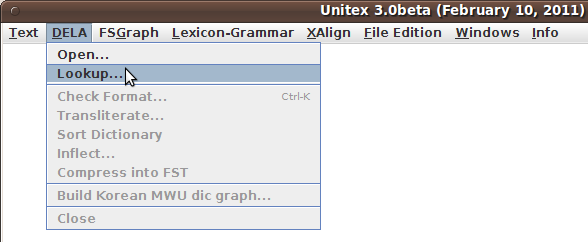
\includegraphics[width=13cm]{resources/img/fig3-1.png}
\caption{"DELA" Menu}
\end{center}
\end{figure}

\bigskip
\noindent
If you have opend a dictionary, the displayed window contains a field where you can enter a word to search. If the word appears in the dictionary, the Find Button will highlight the first entry that matches it. If there is several entries for this word, you can browse all matches by clicking on the two arrow buttons.

\begin{figure}[h!]
\begin{center}
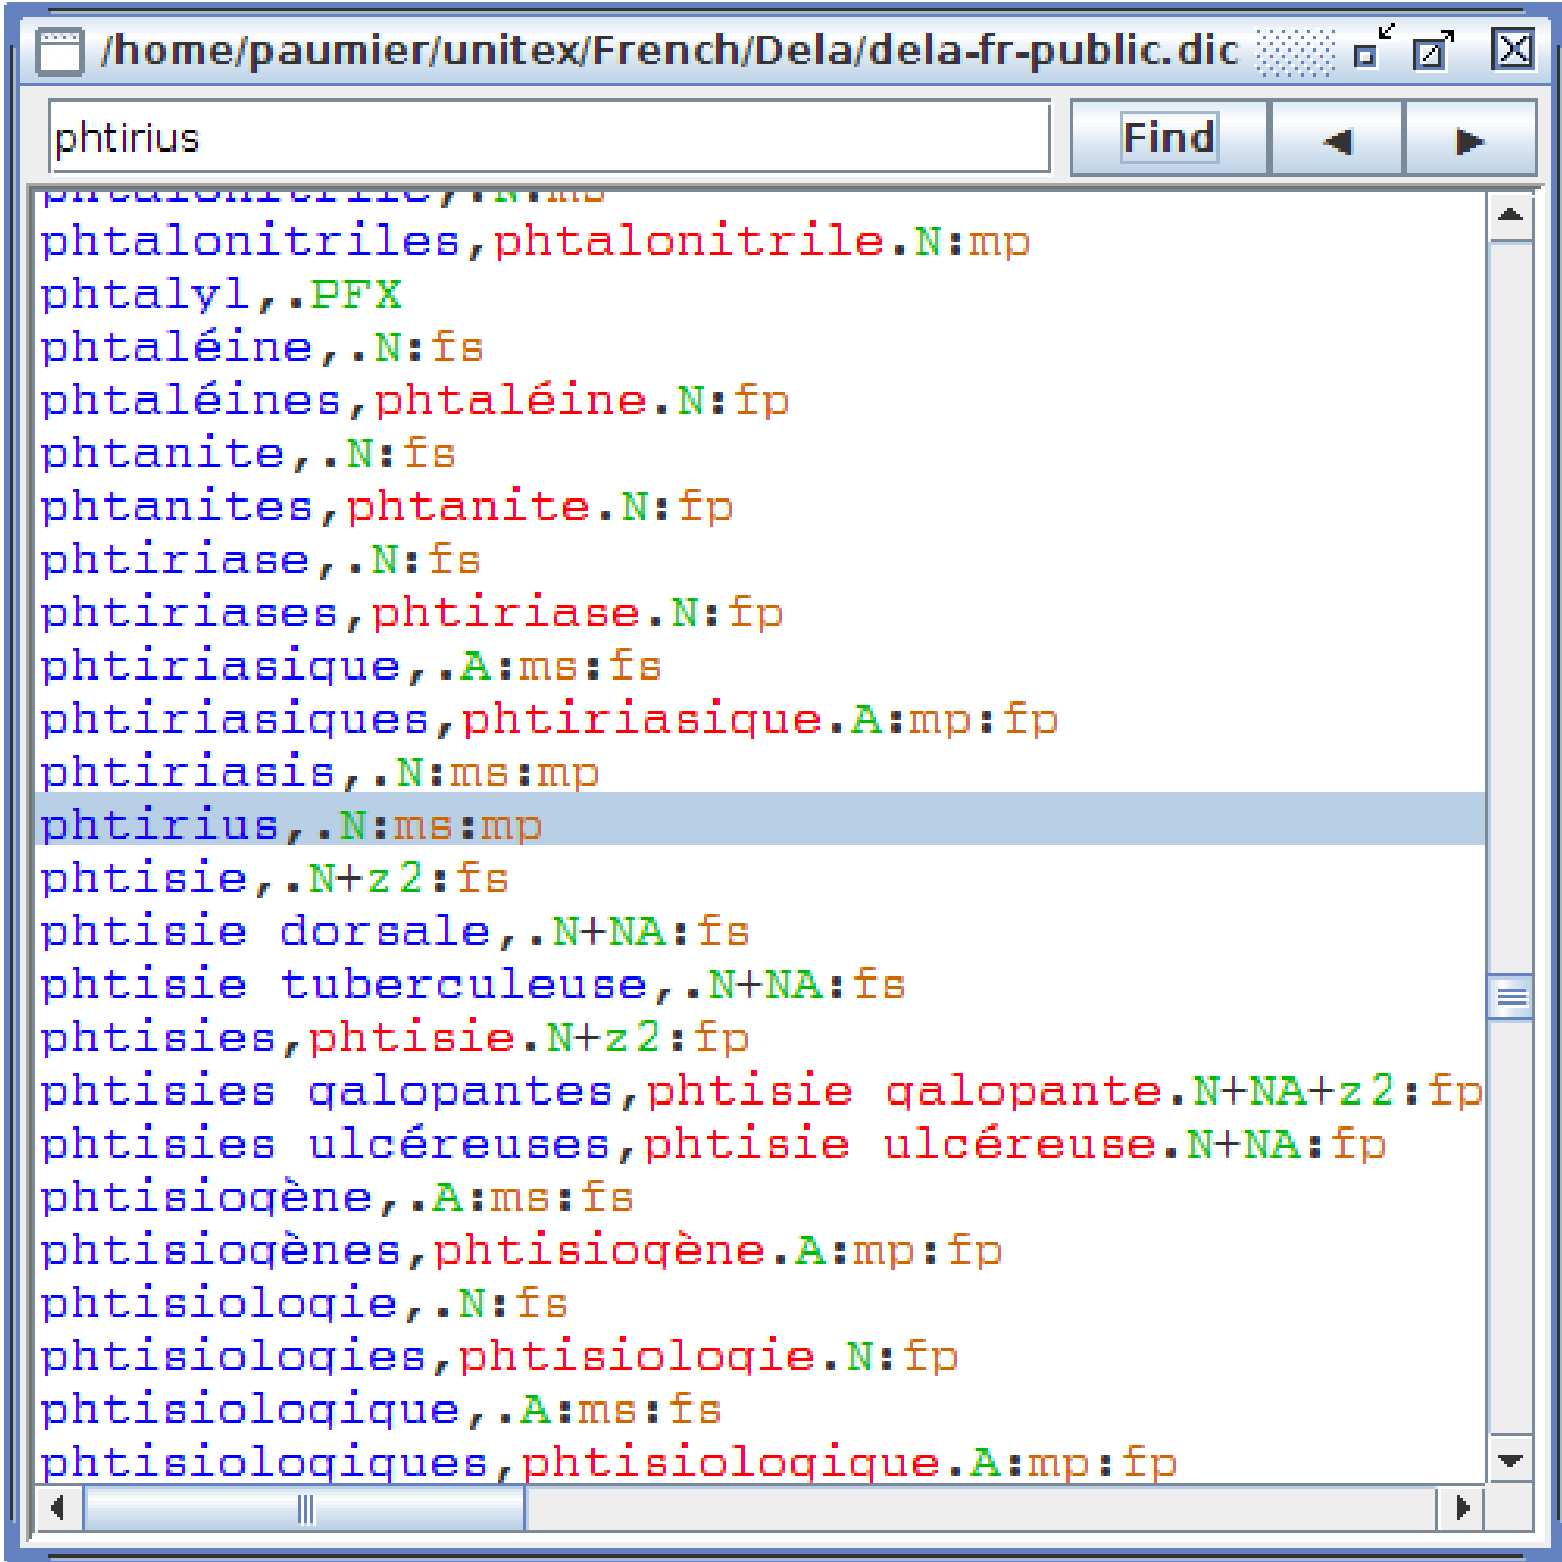
\includegraphics[width=7cm]{resources/img/fig3-2.png}
\caption{Looking up for a word in a dictionnary}
\end{center}
\end{figure}

\bigskip
\noindent
You can also look up a word in several dictionnaries by clicking on the Lookup button of the DELA menu. You can then select the dictionaries in which you want to look up the word you have entered.

\begin{figure}[h!]
\begin{center}
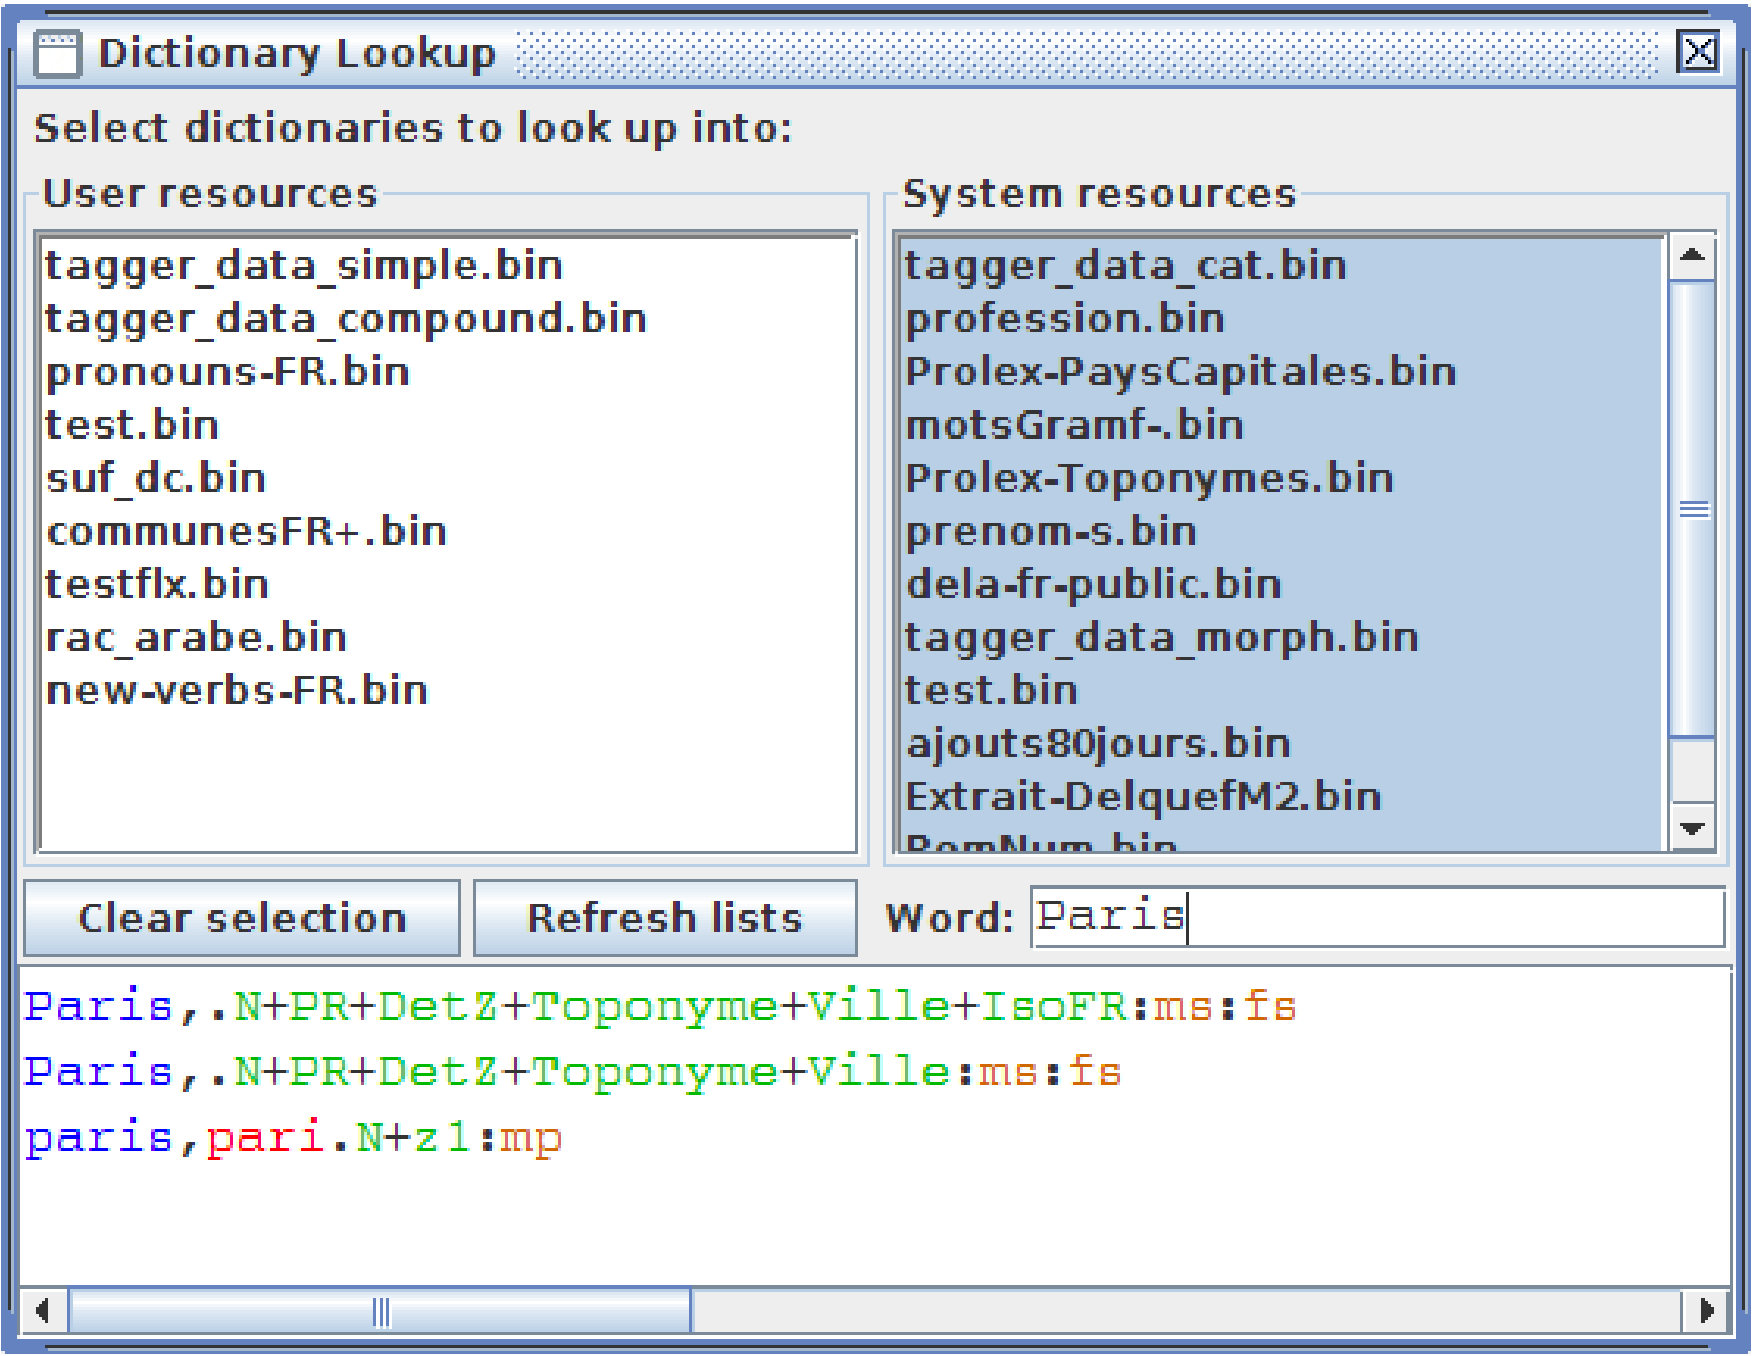
\includegraphics[width=7cm]{resources/img/fig3-3.png}
\caption{Looking up for a word in several dictionnaries}
\end{center}
\end{figure}

\bigskip
\noindent

%%%%%%%%%%%%%%%%%%
\section{Checking dictionary format}
\index{Dictionaries!checking} \index{Checking dictionary format}
When dictionaries become large, it becomes tiresome to check them by hand.
Unitex contains the program \verb+CheckDic+\index{External
programs!\verbc{CheckDic}}\index{\verbc{CheckDic}} that automatically checks the
format of DELAF and DELAS dictionaries.

\bigskip
\noindent This program verifies the syntax of the entries. For each malformed
entry the program outputs the line number, the content of the line and an error
message. Results are saved in the file
\verb+CHECK_DIC.TXT+\index{File!\verbc{CHECK_DIC.TXT}} which is displayed when the
verification is finished. In addition to eventual error messages, the file also
contains the list of all characters used in the inflectional and canonical forms,
the list of grammatical and semantic codes, and the list of inflectional codes
that appear in the dictionary. The character list makes it possible to verify
that the characters used in the dictionary are consistent with those in the 
alphabet file of the language. Each character is followed by its value in hexadecimal
notation.\index{File!alphabet}

\bigskip
\noindent The code lists can be used to check that there are no typing errors 
in the codes of the dictionary.

\bigskip
\noindent The \verb+CheckDic+ program works with non-compressed dictionaries,
\textit{i.e.} the files in text format. The general convention is to use the
\verb+.dic+ extension for these dictionaries. In order to check the 
\index{File!\verbc{.dic}} format of a
dictionary, you first open it by choosing "Open..." in the "DELA" menu.

\begin{figure}[!ht]
\begin{center}
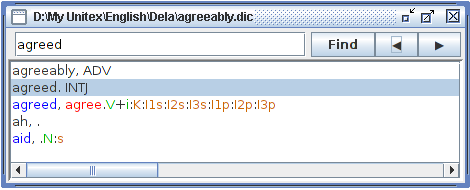
\includegraphics[width=10cm]{resources/img/fig3-4.png}
\caption{Dictionary example\label{fig-dictionary-example}}
\end{center}
\end{figure}

\noindent Let's load the dictionary as in figure~\ref{fig-dictionary-example}.
Then, click on "Check Format..." in the
"DELA" menu. A window like in
figure~\ref{fig-dictionary-checking} is opened. You
must select the type of dictionary you want to check. After checking the dictionary in Figure~\ref{fig-dictionary-example}, 
results are presented as shown in Figure~\ref{fig-dictionary-checking-results}.

\begin{figure}[!ht]
\begin{center}
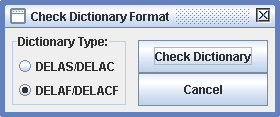
\includegraphics[width=7cm]{resources/img/fig3-5.png}
\caption{Checking a dictionary\label{fig-dictionary-checking}}
\end{center}
\end{figure}

\begin{figure}[!p]
\begin{center}
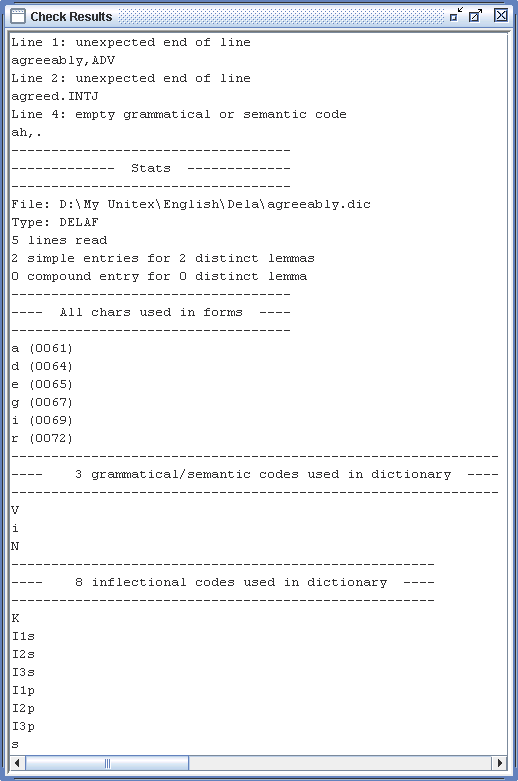
\includegraphics[height=19.4cm]{resources/img/fig3-6.png}
\caption{Results of checking\label{fig-dictionary-checking-results}}
\end{center}
\end{figure}

\bigskip
\noindent The first error is caused by a missing period. The second, by the fact
that no comma was found after the end of an inflected form. The third error indicates
that the program didn't find any grammatical or semantic codes.


\section{Sorting}
\index{Dictionaries!sorting}\index{Sorting!a dictionary}

Unitex uses the dictionaries without having to worry about the order of the
entries. When displaying them it is sometimes preferable to sort the
dictionaries. The sorting depends on a number of criteria, first of all on the
language of the text. Therefore the sorting of a Thai dictionary is done
according to an order different from the alphabetical order.  So different in
fact that Unitex uses a sorting procedure developed specifically for Thai (see
chapter \ref{chap-external-programs}).

\bigskip
\noindent For European languages the sorting is usually done according to the
lexicographical order, although there are some variants. Certain languages like
French treat some characters as equivalent. For example, the difference between
the characters  \verb+e+  and \texttt{\'e}  is ignored if one wants to compare
the words \verb+manger+ et \texttt{mang\'es} because the contexts
\verb+r+ and \verb+s+ allow to decide the order. The difference is only taken 
into account when the contexts are
identical, as they are when comparing \texttt{p\^eche} and
\texttt{p\`eche}.

\bigskip \index{Alphabet!sort}
\noindent
To allow for such effect, the \verb+SortTxt+ program  
\index{\verbc{SortTxt}}\index{External programs!\verbc{SortTxt}} uses a file which
defines the equivalence of characters. \index{Equivalent characters}  This file
is named \verb+Alphabet_sort.txt+ \index{File!\verbc{Alphabet_sort.txt}} and can
be found in the user directory for the current language. By default the first
lines of this file for French look like this:

\bigskip
\begin{minipage}{\textwidth}
\noindent\texttt{A\`A\^A\"Aa\`a\^a\"a}

\noindent\texttt{Bb}

\noindent\texttt{C\c{C}c\c{c}}

\noindent\texttt{Dd}

\noindent\texttt{E\'E\`E\^E\"Ee\'e\`e\^e\"e}
\end{minipage}

\bigskip
\noindent Characters in the same line are considered equivalent if the context permits. If
two equivalent characters must be compared, they are sorted in the order they
appear in from left to right. As can be seen from the extract above, there is no
difference between lower and upper case. Accents and the c\'edille character are
ignored as well.

\bigskip
\noindent To sort a dictionary, open it and then click on "Sort Dictionary" in
 the "DELA" menu. By default, the program always looks for the file
\verb+Alphabet_sort.txt+. If that file doesn't exist, the sorting is done
according to the character indices in the Unicode encoding. By modifying that
file, you can define your own sorting order.

\bigskip
\noindent NOTE: After applying the dictionaries to a text, the files
\verb+dlf+, \verb+dlc+ and \verb+err+ are automatically sorted using this
program. \index{File!\verbc{dlf}} \index{File!\verbc{dlc}}
\index{File!\verbc{err}}



\section{Automatic inflection}
\label{section-automatic-inflection}
\index{Inflection}\index{Conjugation}\index{Declension}\index{Automatic inflection}\index{Dictionaries!automatic inflection}
\subsection{Inflection of simple words}

As described in section~\ref{section-DELAS-format}, a line in a DELAS
consists of a canonical form and a sequence of grammatical or semantic codes:

\begin{verbatim}
aviatrix,N4+Hum
matrix,N4+Math
radix,N4
\end{verbatim}

\bigskip
\noindent The first code is used to determine the grammatical code of the entry as
well as the name of the grammar used to inflect the canonical form. There are
two possible forms:

\begin{itemize}
  \item \verb+N4+: grammar name=\verb+N4.fst2+, grammatical code=\verb+N+
  (longest letter prefix)
  \item \verb+N(NC_XXX)+: grammar name=\verb+NC_XXX.fst2+, grammatical code=\verb+N+
\end{itemize}

\bigskip
\noindent These inflectional grammars \index{Grammars!inflectional}\index{Transducer!inflection}\index{Graph!inflection}
will automatically be
compiled if needed. In the example above, all entries will be inflected by a grammar named \verb+N4+.

\bigskip
\noindent In order to  inflect a dictionary, click on "Inflect..." in the "DELA" menu. The
window in figure~\ref{fig-inflection-configuration} allows you to specify the
directory in which inflectional grammars are found. By default, the subdirectory
\verb+Inflection+ of the directory for the current language is used. You can
also specify the kind of words your DELAS is supposed to contain. If an entry is
found that does not correspond to your choice, an error message will be
displayed.

\bigskip
\begin{figure}[!ht]
\begin{center}
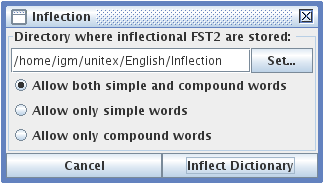
\includegraphics[width=8cm]{resources/img/fig3-7.png}
\caption{Configuration of automatic inflection\label{fig-inflection-configuration}}
\end{center}
\end{figure}

\bigskip
\begin{figure}[!ht]
\begin{center}
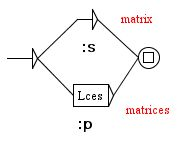
\includegraphics[width=4.5cm]{resources/img/fig3-8.png}
\caption{Inflectional grammar
\texttt{N4}\label{fig-example-inflectional-grammar}}
\end{center}
\end{figure}

\bigskip
\noindent Figure~\ref{fig-example-inflectional-grammar} shows an example of an
inflectional grammar. The paths describe the suffixes to add or to remove to
get to an inflected form from a canonical form, and the outputs (text in bold under the boxes) are the
inflectional codes to add to a dictionary entry.

\bigskip
\noindent In our example, two paths are possible. The first does not modify the
canonical form and adds the inflectional code \verb+:s+. The second deletes a letter with
the \verb+L+ operator, then adds the \verb+ces+ suffix and adds the inflectional
code \verb+:mp+. Here are the operators that can be used:

\begin{itemize}
  \item \verb+L+ (left) removes a letter from the entry.\index{\verbc{L}}\index{Operator!\verbc{L}}
  
  \item \verb+R+ (right) restores a letter to the entry.\index{\verbc{R}}\index{Operator!\verbc{R}}
  In French, many verbs
  of the first group are conjugated in the present singular  of the third person form  by removing the
  \verb+r+ of the infinitive and changing the 4$^{th}$ letter from the end to
  \texttt{\`e}: \verb+peler+ $\rightarrow$ \texttt{p\`ele},
  \verb+acheter+ $\rightarrow$ \texttt{ach\`ete}, \texttt{g\'erer}
  $\rightarrow$ \texttt{g\`ere}, etc. Instead of describing an inflectional
  suffix for each verb (\texttt{LLLL\`ele}, \texttt{LLLL\`ete} and
  \texttt{LLLL\`ere}), the \verb+R+ operator can be used to
  describe it in one way: \texttt{LLLL\`eRR}.
  
  \item \verb+C+ (copy)\index{\verbc{C}}\index{Operator!\verbc{C}}
  duplicates a letter in the entry and moves everything on
  its right by one position. In cases like \verb+permitted+ or \verb+hopped+, we
  see a duplication of the final consonant of the verb. To avoid writing an
  inflectional graph for every possible final consonant, one can use the \verb+C+
  operator to duplicate any final consonant.
  
  \item \verb+D+ (delete)\index{\verbc{D}}\index{Operator!\verbc{D}} deletes a
  letter, shifting anything located on the right of this letter. For instance, if
  you want to inflect the Romanian word \verb+european+ into \verb+europeni+, you
  must use the sequence \verb+LDRi+. \verb+L+ will move the cursor on the
  \verb+a+, \verb+D+ will delete the \verb+a+, shifting the \verb+n+ on the left,
  and then \verb+Ri+ will restore the \verb+n+ and add an \verb+i+.

  \item \verb+U+ (unaccent)\index{\verbc{U}}\index{Operator!\verbc{U}}
  removes the accent of the current character, if
  any. For instance the sequence \verb+LLUx+ applied to the word
  \texttt{mang\'es} produces the inflected form \verb+mangex+, since \verb+U+
  has turn the \texttt{\'e} into a \verb+e+.

  \item \verb+P+ (uppercase)\index{\verbc{P}}\index{Operator!\verbc{P}}
  uppercases the initial letter of the stack. For
  instance, the sequence \verb$Px$ will turn \verb$foo$ into \verb$Foox$.
  
  \item \verb+W+ (lowercase)\index{\verbc{W}}\index{Operator!\verbc{W}}
  lowercases the initial letter of the stack.

  \item \verb+<R=?>+ \index{\verbc{<R=?>}}\index{Operator!\verbc{<R=?>}}
  replaces the initial letter of the stack by the letter \verb+?+.

  \item \verb+<I=?>+ \index{\verbc{<I=?>}}\index{Operator!\verbc{<I=?>}}
  inserts the letter \verb+?+ before the initial letter of the stack. 

  \item \verb+<X=n>+ \index{\verbc{<X=n>}}\index{Operator!\verbc{<X=n>}}
  removes the first $n$ letters of the stack. 
   
\end{itemize}

\noindent There are also two operators dedicated to Korean:
\begin{itemize}\index{Jamo}\index{Hangul}
    \item \verb+J+ removes a Jamo letter.\index{\verbc{J}}\index{Operator!\verbc{J}}
    If the current character is a Hangul
    syllab character, this character is first replaced by the equivalent Jamo
    sequence, and then, the last Jamo letter is removed. If the current
    character is neither a Jamo nor a Hangul, and error is raised.
    
    \item \verb+.+ (latin dot)\index{\verbc{.}}\index{Operator!\verbc{.}}
    inserts a syllab bound. As a side effect, if the
    top of the stack contains Jamo letters, they are first recombined into a
    Hangul character.
    \end{itemize}


\bigskip
\noindent In the example below, the inflection of \verb+choose+ is
shown. The sequence \verb+LLDRRn+ describes the form \verb+chosen+:

\begin{itemize}
  \item Step 0: the canonical form is copied on the stack, and the cursor is set behind the last letter:
  
  \begin{center}
\begin{tabular}{|l|l|l|l|l|l|l|l}
\multicolumn{6}{l}{} & \multicolumn{2}{l}{$\downarrow$} \\
\hline
\verb+c+ & \verb+h+ & \verb+o+ & \verb+o+ & \verb+s+ & \verb+e+ & \verb+ + & \\
\hline
\end{tabular}
\end{center}

\bigskip
\item Step 1: the cursor is moved one position to the left:

\begin{center}
\texttt{\textbf{L}LDRRn}

\begin{tabular}{|l|l|l|l|l|l|l|l}
\multicolumn{5}{l}{} & \multicolumn{3}{l}{$\downarrow$} \\
\hline
\verb+c+ & \verb+h+ & \verb+o+ & \verb+o+ & \verb+s+ & \verb+e+ & \verb+ + & \\
\hline
\end{tabular}
\end{center}

\bigskip
\item Step 2: the cursor is moved one position to the left again:

\begin{center}
\texttt{\textbf{LL}DRRn}

\begin{tabular}{|l|l|l|l|l|l|l|l}
\multicolumn{4}{l}{} & \multicolumn{4}{l}{$\downarrow$} \\
\hline
\verb+c+ & \verb+h+ & \verb+o+ & \verb+o+ & \verb+s+ & \verb+e+ & \verb+ + & \\
\hline
\end{tabular}
\end{center}

\bigskip \item Step 3: one character is deleted; everything to the right of the
cursor is shifted one position to the left:

\begin{center}
\texttt{\textbf{LLD}RRn}

\begin{tabular}{|l|l|l|l|l|l|l|l}
\multicolumn{3}{l}{} & \multicolumn{5}{l}{$\downarrow$} \\
\hline
\verb+c+ & \verb+h+ & \verb+o+ & \verb+s+ & \verb+e+ & \verb+ + & \verb+ + & \\
\hline
\end{tabular}
\end{center}

\bigskip
\item Step 4: the cursor is moved to the right:

\begin{center}
\texttt{\textbf{LLDR}Rn}

\begin{tabular}{|l|l|l|l|l|l|l|l}
\multicolumn{4}{l}{} & \multicolumn{4}{l}{$\downarrow$} \\
\hline
\verb+c+ & \verb+h+ & \verb+o+ & \verb+s+ & \verb+e+ & \verb+ + & \verb+ + & \\
\hline
\end{tabular}
\end{center}

\bigskip
\item Step 5: and to the right again:

\begin{center}
\texttt{\textbf{LLDRR}n}

\begin{tabular}{|l|l|l|l|l|l|l|l}
\multicolumn{5}{l}{} & \multicolumn{3}{l}{$\downarrow$} \\
\hline
\verb+c+ & \verb+h+ & \verb+o+ & \verb+s+ & \verb+e+ & \verb+ + & \verb+ + & \\
\hline
\end{tabular}
\end{center}

\bigskip
\item Step 6: the character \verb+n+ is pushed on the stack:

\begin{center}
\texttt{\textbf{LLDRRn}}

\begin{tabular}{|l|l|l|l|l|l|l|l}
\multicolumn{6}{l}{} & \multicolumn{2}{l}{$\downarrow$} \\
\hline
\verb+c+ & \verb+h+ & \verb+o+ & \verb+s+ & \verb+e+ & \verb+n+ & \verb+ + & \\
\hline
\end{tabular}
\end{center}
\end{itemize}

\bigskip
\noindent When all operations have been fulfilled, the inflected form
consists of all letters before the cursor (here \verb+chosen+).

\bigskip
\noindent The inflection program
explores all paths of the inflectional grammar and tries all possible forms. In
order to avoid having to replace the names of inflectional grammars by the actual
grammatical codes to be used in the dictionary, the program replaces these names by the
longest prefixes made of letters.
% if you have selected the "Remove class numbers" button.
Thus, \verb+N4+ is replaced by \verb+N+. By choosing the inflectional
grammar names carefully, one can construct a ready-to-use dictionary.

\bigskip
\noindent Figure \ref{fig-inflection-result} shows the dictionary we get after the inflection of 
our DELAS example.

\bigskip
\begin{figure}[!ht]
\begin{center}
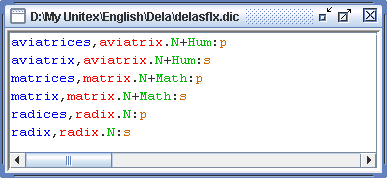
\includegraphics[width=9.5cm]{resources/img/fig3-9.png}
\caption{Result of automatic inflection\label{fig-inflection-result}}
\end{center}
\end{figure}
\subsection{Advanced inflection operators}
\label{advanced-inflection-operators}

In some languages the inflection process can modify the root of the word.
Several operators have been developped in order to facilitate this type of treatment. 
They allow to find and remove a suffix of the word \verb+W+ to be inflected.
It is also possible to store a factor of this suffix by using a special variable (\$ or ${\pounds}$).
These operators can take the following forms:

\begin{itemize}
\item \verb+<X$Y>+: Starting from the end of the word \verb+W+  we are looking for the suffix \verb+Y+.
	Then, we search for the {\bf rightmost} occurrence of \verb+X+ which strictly precedes that 
	of  \verb+Y+ . The \$ variable then contains the {\bf shortest factor}
	({\bf\$}hortest) of \verb+W+ strictly between \verb+X+ and \verb+Y+ (\verb+W = U.X.$.Y+)\footnote{The point
	represents here the concatenation operation.}.
	The \verb+<X$Y>+ operator strips \verb+X.$.Y+ from \verb+W+ and sets \$. After it has been applied, the string
	left in the stack is \verb+U+, and the \$ variable can be used in the rest of the path.
\item \verb+<X+${\pounds}$\verb+Y>+:  Starting from the end of the word \verb+W+
	we are looking for the suffix \verb+Y+.
	Then, we search for the {\bf leftmost} occurrence of \verb+X+ which strictly precedes that of \verb+Y+.
	The {\pounds}  variable then contains the  {\bf longest factor}
	({\bf${\pounds}$}ongest) of \verb+W+ strictly between
	\verb+X+ and \verb+Y+ (\verb+W = U.X.+${\pounds}$\verb+.Y+).
\item \verb+<X>+: If there is no variable, we search for \verb+X+ as a suffix of \verb+W+
	(\verb+W = U.X+).
\item \verb+<$Y>+: If the \verb+X+ factor is absent,
	the {\bf shortest factor \verb+$+} is the first letter which strictly precedes \verb+Y+ .
\item \verb+<+${\pounds}$\verb+Y>+: If the \verb+X+ factor is absent,
	the {\bf longest factor ${\pounds}$} is the prefix of
	\verb+W+ so that  \verb+W = +${\pounds}$ \verb+.Y+.
\end{itemize}

\noindent
To illustrate the use of these operators, let us consider the French verb {\it reprendre}:

\bigskip
\begin{center}
\begin{tabular}{|l|l|l|l|}
\hline
Word     & Operator & Variable & Result\\
\hline
\hline
reprendre & <re> & & reprend\\
reprendre & <\$> & \$ = e & reprendr\\
reprendre & <{\pounds}> &{\pounds}= reprendre & $\varepsilon$ \\
reprendre & <re\$re> & \$ = nd & rep\\
reprendre & <re{\pounds}re> & {\pounds} = prend & \\
reprendre & <\$re> & \$ = d & repren\\
reprendre & <re\$> & \$ =  $\varepsilon$ & reprendre\\
reprendre & <{\pounds}re> & {\pounds} = reprend & $\varepsilon$\\
reprendre & <re{\pounds}> & {\pounds} = prendre & re\\
\hline
\end{tabular}
\end{center}

\bigskip
\noindent
The MultiFlex program allows you to use ten variables of type \$ whose names are \$,\$1,...,\$9
and ten variables of type {\pounds} whose names are {\pounds},{\pounds}1,...,{\pounds}9.
Morever, both types of variables can be mixed in a same operator. Thus the operator <{\pounds}3re\$7re>
applied to the french verb {\it reprendre} gives back~: {\pounds}3 = rep et \$7 = \verb+nd+.

\bigskip
\noindent
In the verbs \verb+accélérer+, \verb+sécher+, the second person of the present tense
can be generated by the operation <é\$er>è\$es~:

\begin{center}
\begin{tabular}{lllllllll}
	\verb+accélérer+ & <é\$er> & $\rightarrow$ & accél & \$ = r & + & è\$es &  $\rightarrow$ & \verb+accélères+\\
	\verb+sécher+ & <é\$er> & $\rightarrow$ & s & \$ = ch & + & è\$es & $\rightarrow$ & \verb+sèches+\\
\end{tabular}
\end{center}

%\bigskip
\noindent
Note that the factor \verb+$+ which remains in the inflected form is of variable length (\verb+r+, \verb+ch+). 
The inflection of the verbs \verb+accélérer+ and \verb+sécher+ cannot be done with classical stack operators
within the same operation. Two different operations (\verb+-4RèCes+, \verb+-5RèCes+) are
needed. The graph shown in figure~\ref{fig-inflection-secher} inflects verbs like
\verb+accélérer+ and \verb+sécher+ in the present tense.

%\bigskip
\begin{figure}[!ht]
\begin{center}
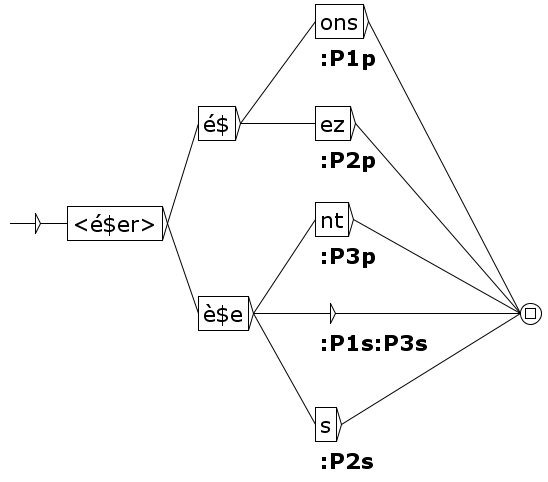
\includegraphics[width=7cm]{resources/img/fig3-Advanced_operators_with_Variables-V_secher.png}
\caption{Inflection graph for verbs like {\it accélérer}, {\it sécher}
\label{fig-inflection-secher}}
\end{center}
\end{figure}

\newpage
%\bigskip
\noindent
The inflected forms of the verbs \verb+accélérer+ and \verb+sécher+ are~:

%\bigskip
\begin{figure}[!ht]
\begin{center}
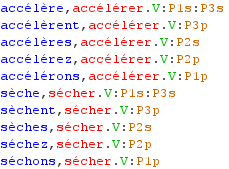
\includegraphics[width=5cm]{resources/img/fig3-flexion_secher.png}
\end{center}
\end{figure}

\bigskip
\noindent
The doubling of some letters during the inflection process can be done with the operator \$.
For example the adjective {\it tranquil} has two forms in the comparative and two in the 
superlative. The graph in figure ~\ref{fig-inflection-tranquil} can produce these forms.

\bigskip
\begin{figure}[!ht]
\begin{center}
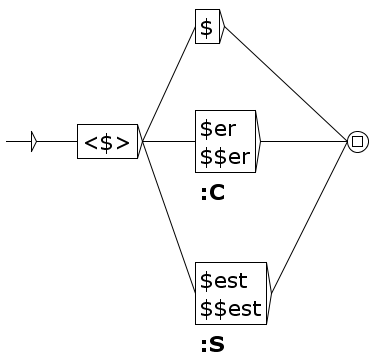
\includegraphics[width=5.5cm]{resources/img/fig3-Advanced_operators_with_Variables-A_tranquil.png}
\caption{Inflection graph for adjectives like {\it tranquil}
\label{fig-inflection-tranquil}}
\end{center}
\end{figure}

\noindent Below are the inflected forms for the adjective \verb+tranquil+~:

\bigskip
\begin{figure}[!ht]
\begin{center}
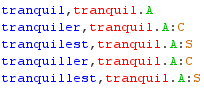
\includegraphics[width=5cm]{resources/img/fig3-flexion_tranquil.png}
\end{center}
\end{figure}

%\bigskip
\noindent  In some languages, some inflected forms have a prefix added before the root like the formation of the past participle in German. The joint use of operators
${\pounds}$ et \verb+$+ allows to inflect the german verb \verb+sprechen+ (to speak)
in the present tense and the past participle as shown in the graph in figure~\ref{fig-inflection-sprechen}.

\newpage
%\bigskip
\begin{figure}[!htbp]
\begin{center}
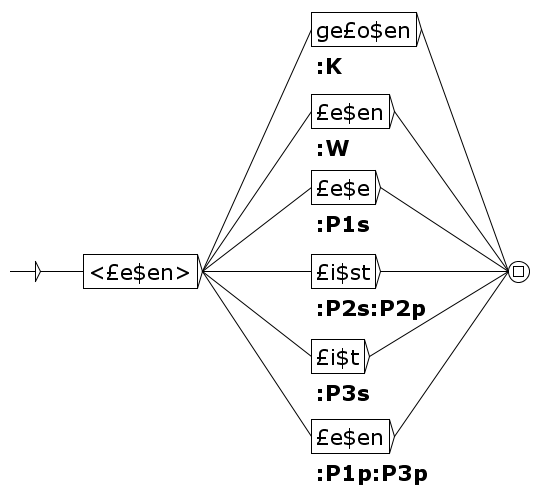
\includegraphics[width=5cm]{resources/img/fig3-Advanced_operators_with_Variables-V_sprechen.png}
\caption{Inflection graph for verbs like {\it sprechen}
\label{fig-inflection-sprechen}}
\end{center}
\end{figure}

%\bigskip
\noindent The inflection forms of the verb \verb+sprechen+~:

\bigskip
\begin{figure}[!ht]
\begin{center}
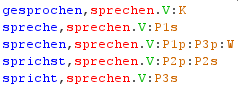
\includegraphics[width=5cm]{resources/img/fig3-flexion_sprechen.png}
\end{center}
\end{figure}

%\bigskip
\noindent In order to inflect the phrasal verb  \verb+aussprechen+  two variables of type \$ should be used.
Figure ~\ref{fig-inflection-aussprechen} shows a graph with two variables \verb+$1+ and \verb+$2+.

\bigskip
\begin{figure}[!ht]
\begin{center}
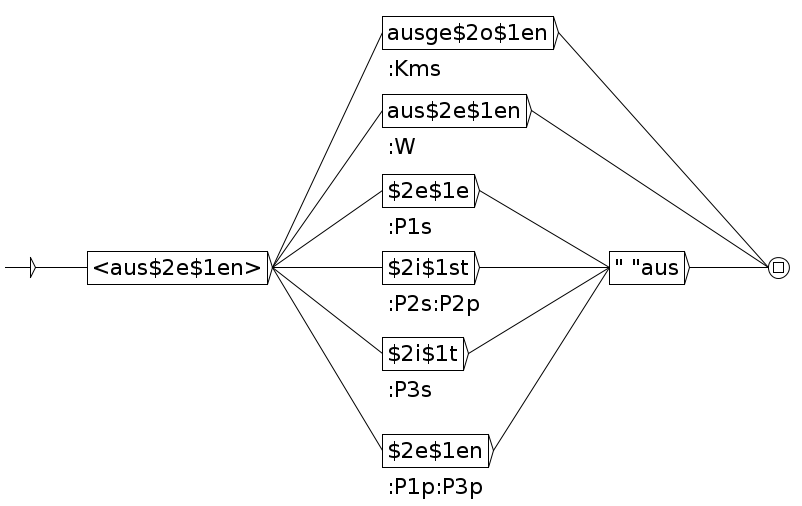
\includegraphics[width=10.5cm]{resources/img/fig3-Advanced_operators_with_Variables-V_aussprechen.png}
\caption{Inflection graph for verbs like {\it aussprechen}
\label{fig-inflection-aussprechen}}
\end{center}
\end{figure}

\noindent Here are the inflection forms of the verb \verb+aussprechen+~:
\bigskip
\begin{figure}[!ht]
\begin{center}
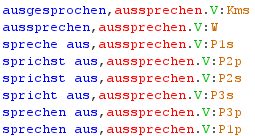
\includegraphics[width=5cm]{resources/img/fig3-flexion_aussprechen2.png}
\end{center}
\end{figure}

\bigskip
\noindent \textbf{Semantic codes}

\noindent In some languages, there are inflectional features that actually correspond to 
semantic ones, like for instance markers for the passive form. Such codes may not appear
as inflectional ones, but rather as semantic ones. To do that and produce semantic codes, 
you have to insert a plus sign at the beginning of the output of a box. The box must only 
contain the semantic code preceeded by a plus, as shown on Figure \ref{fig-inflection-sem}.

\bigskip
\begin{figure}[!ht]
\begin{center}
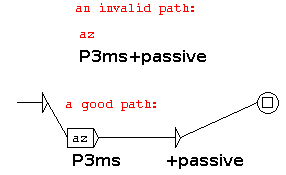
\includegraphics[width=6cm]{resources/img/fig3-9sem.png}
\caption{An inflection grammar with a semantic code\label{fig-inflection-sem}}
\end{center}
\end{figure}


\subsection{Inflection of compound words}
See chapter \ref{chap-multiflex}.


\subsection{Inflection of Semitic languages}
\label{subsection-semitic-inflection}
\index{Semitic languages}
Semitic languages like Arabic or Hebrew are inflected in a way not easily representable 
with the inflection operators described above. Their morphology obeys a different logic:
words are inflected according to \textit{consonant
skeletons}\index{Consonant skeleton}. The inflection process combines this skeleton with vowels.
Specific operators have been implemented for Semitic languages, and some of them may be useful
also for languages outside the Semitic family, such as Tagalog.

\bigskip
\noindent First, let us see a case where we encode only the consonants in the lemma field of the DELAS  entry:

\bigskip
\noindent \verb+ktb,$V31-123+

\bigskip
\noindent The \verb+$+ sign before the grammatical code indicates that the inflection grammar 
is in the Semitic mode, and the form \verb+ktb+ in the lemma field is the consonant
skeleton. Figure~\ref{semitic-grammar} shows the toy grammar \verb+V31-123.grf+
that illustrates how the Semitic mode works. The inflection grammars use the Buckwalter++
transliteration of the Arabic script (cf.~Section~\ref{transliteration-Arabic}).

\bigskip
\begin{figure}[!ht]
\begin{center}
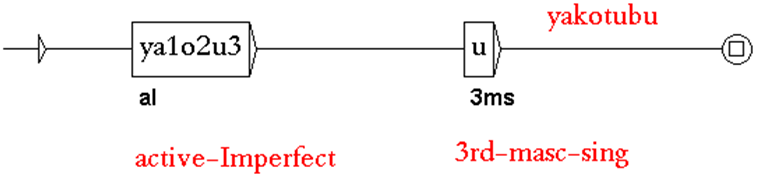
\includegraphics[width=10cm]{resources/img/fig3-15.png}
\caption{A toy inflection grammar\label{semitic-grammar} in the Semitic mode}
\end{center}
\end{figure}

\noindent The Semitic mode obeys the following rules:
\begin{enumerate}
  \item All standard inflection operators can be used (\verb+L+, \verb+R+, etc.).
  \item A digit stands for a letter in the lemma field (\verb+1+ for the first,
  \verb+2+ for the second, etc.). In our example, \verb+1+, \verb+2+ and
  \verb+3+ will respectively stand for \verb+k+, \verb+t+ and
  \verb+b+. If you want to access to a letter after the ninth one, you must
  protect its index with angles like \verb+<10>+.
\end{enumerate}  

\noindent The DELAF output for this grammar is:
  
\verb+yakotubu,ktb.V:aI3ms+

\bigskip
\noindent If we encode only the consonants in the lemma field and  two entries have the same consonants
but differ in the vowels, we must encode the vowels in the inflection grammars:

\verb+Hsb,$V3au	// to count, Hasaba, yaHosubu+

\verb+Hsb,$V3ii	// to think, Hasiba, yaHosibu+

\begin{figure}[!ht]
\begin{center}
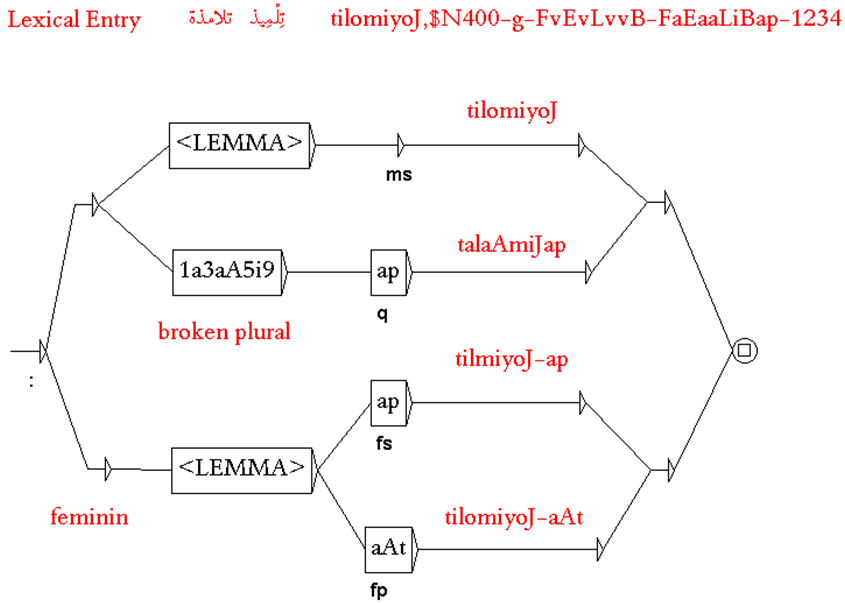
\includegraphics[width=10cm]{resources/img/fig3-LEMMA-operator.png}
\caption{An inflection grammar in the Semitic mode with the <LEMMA> operator\label{LEMMA-operator}}
\end{center}
\end{figure}

\bigskip
\noindent In order to copy the complete lemma field, use the <LEMMA> operator.
A box with this operator retrieves the complete lemma field but does not depend on
the number of letters in the field. This operator is useful for Arabic nouns and adjectives where
masculine forms are generated by inserting vowels in the consonantal skeleton, whereas
feminine forms are obtained by appending suffixes (Figure~\ref{LEMMA-operator}). In this example,
both consonants and vowels are encoded in the lemma field.

\bigskip
\noindent The <n.LEMMA> operator copies the lemma from the $n$th position to the end.
For example, in some Arabic nouns, the short vowel of the first syllable alternates: \verb+a/u+,
\verb+a/i+ or \verb+u/i+, as in \verb+nufaAyap+/\verb+nifaAyap+ ''rubbish''. The inflection grammar of
Fig.~\ref{n.LEMMA-operator} produces both variants with  \verb+u+ and with  \verb+i+ as inflected forms
of \verb+nufaAyap+.

\begin{figure}[!ht]
\begin{center}
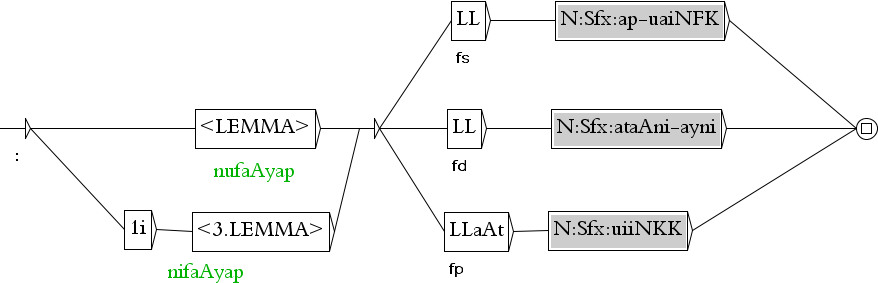
\includegraphics[width=14cm]{resources/img/N0_i_0ap-f-At.png}
\caption{An inflection grammar in the Semitic mode with the <n.LEMMA> operator\label{n.LEMMA-operator}}
\end{center}
\end{figure}

\bigskip
\noindent In Tagalog, an Austronesian language spoken in the Philippines and that uses commonly infixes
and reduplication for inflection, <LEMMA> and <n.LEMMA> may be used to produce verb tenses.
The toy inflection grammar of Fig.~\ref{tagalog} produces the perfect \verb+kumain+, future \verb+kakain+
and imperfect \verb+kumakain+ of the verb \verb+kain+ ''eat''.

\begin{figure}[!ht]
\begin{center}
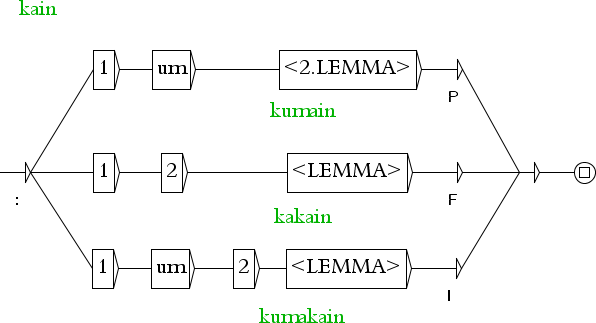
\includegraphics[width=12cm]{resources/img/V1um.png}
\caption{A toy inflection grammar for Tagalog in the Semitic mode\label{tagalog}}
\end{center}
\end{figure}



\section{Transliterating Arabic dictionaries}
\label{transliteration-Arabic}
\index{Transliterating!Arabic}\index{Dictionaries!transliterating}

When Arabic linguists analyse dictionaries in order to spot errors,
reading in the Arabic script is simple and efficient. However, when they
create inflectional grammars (Section~\ref{section-automatic-inflection}), parts of
Arabic words occur in the same box as morphosyntactic information encoded
in the Latin alphabet, and in this context, switching from right-to-left Arabic script
to left-to-right Latin alphabet is a real hassle. With Unitex, you can encode your
inflectional grammars entirely in the Latin alphabet, by using the Buckwalter++
transliteration,\index{Buckwalter++} a one-to-one mapping between a Unicode
encoding of Arabic script and Latin letters (cf.~\cite{neme2011},
Section~3.2, pages~4--6). The Buckwalter++ transliteration is defined by the table
of Fig.~\ref{buckwalter1} and \ref{buckwalter2}.
Unitex provides a tool to internally transliterate DELAS and DELAF Arabic
dictionaries to and from Buckwalter++ encoding
(Fig.~\ref{Arabic-transliteration}). This tool is accessible through the DELA menu.

\begin{figure}[!p]
\centering
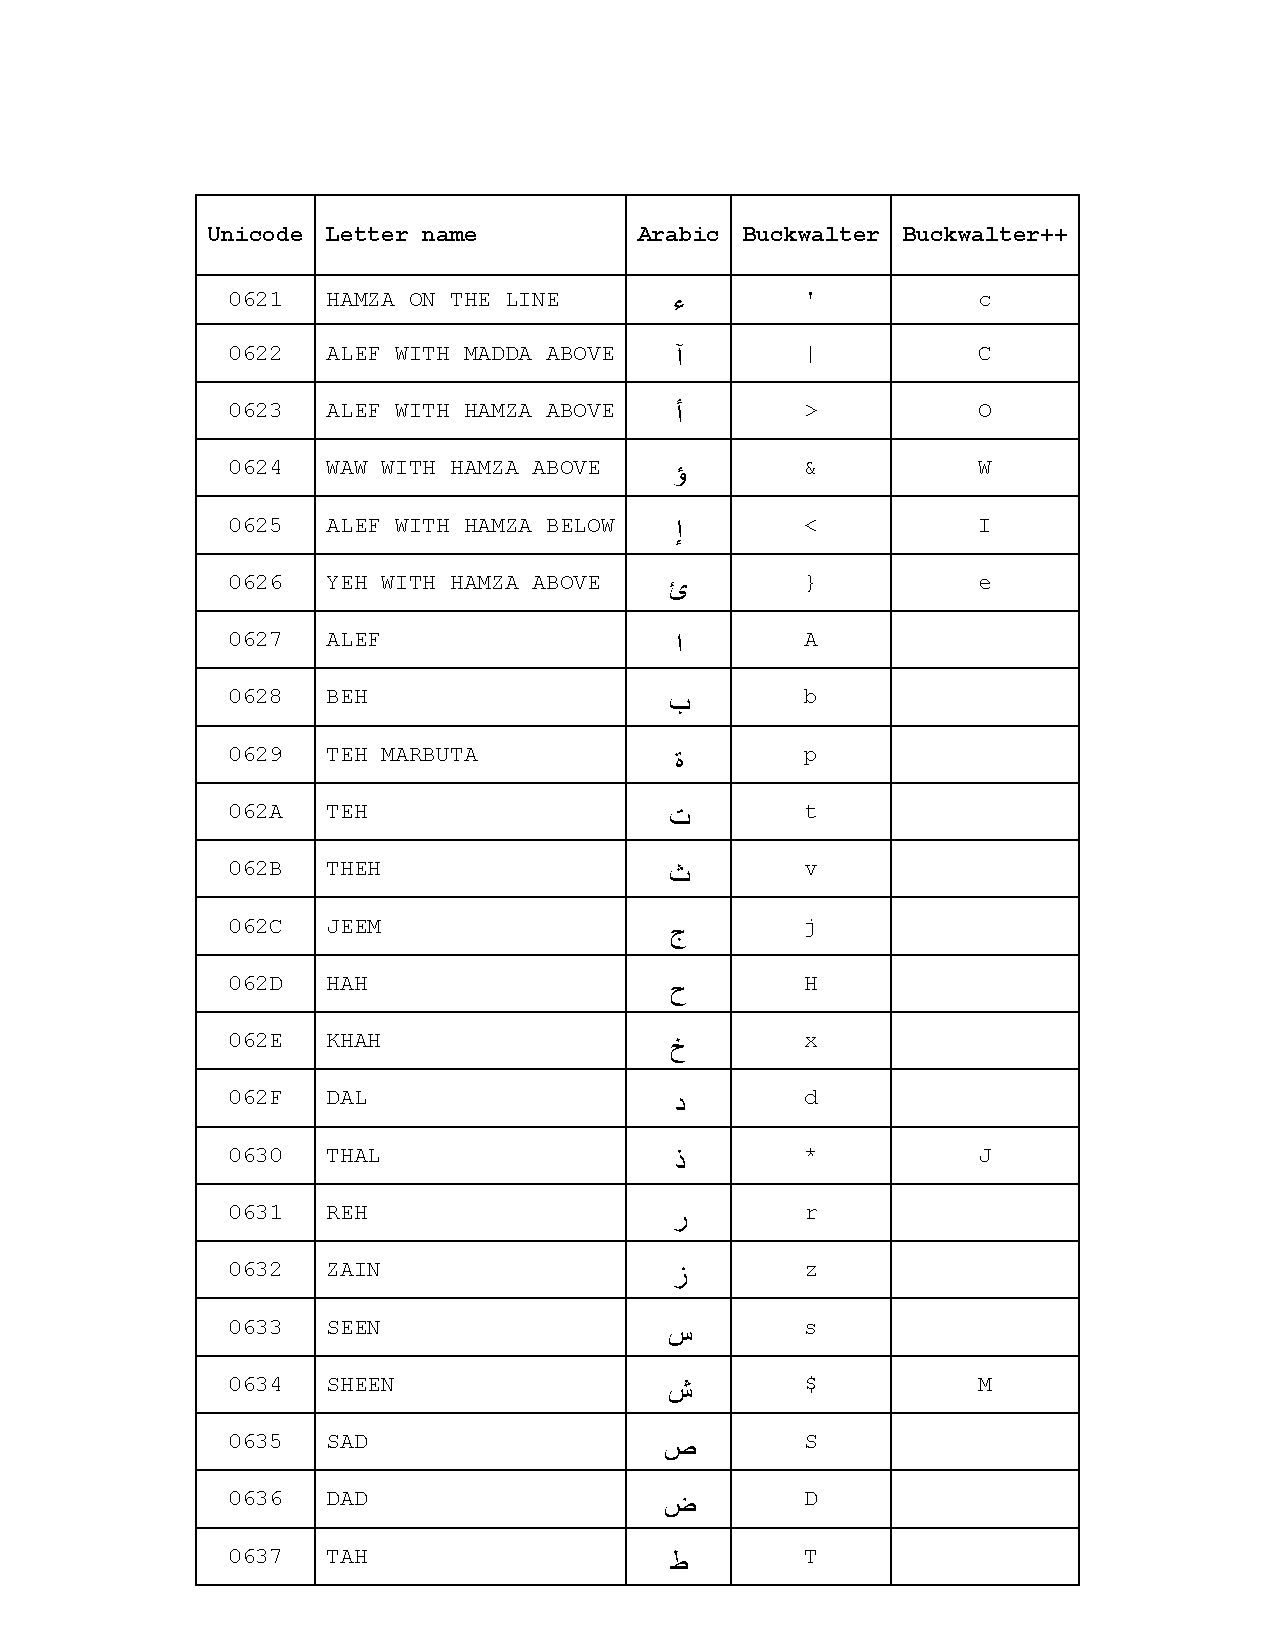
\includegraphics[height=23.5cm]{resources/img/buckwalter1.pdf}
\caption{Buckwalter++ transliteration table, first half\label{buckwalter1}}
\end{figure}

\begin{figure}[!p]
\begin{center}
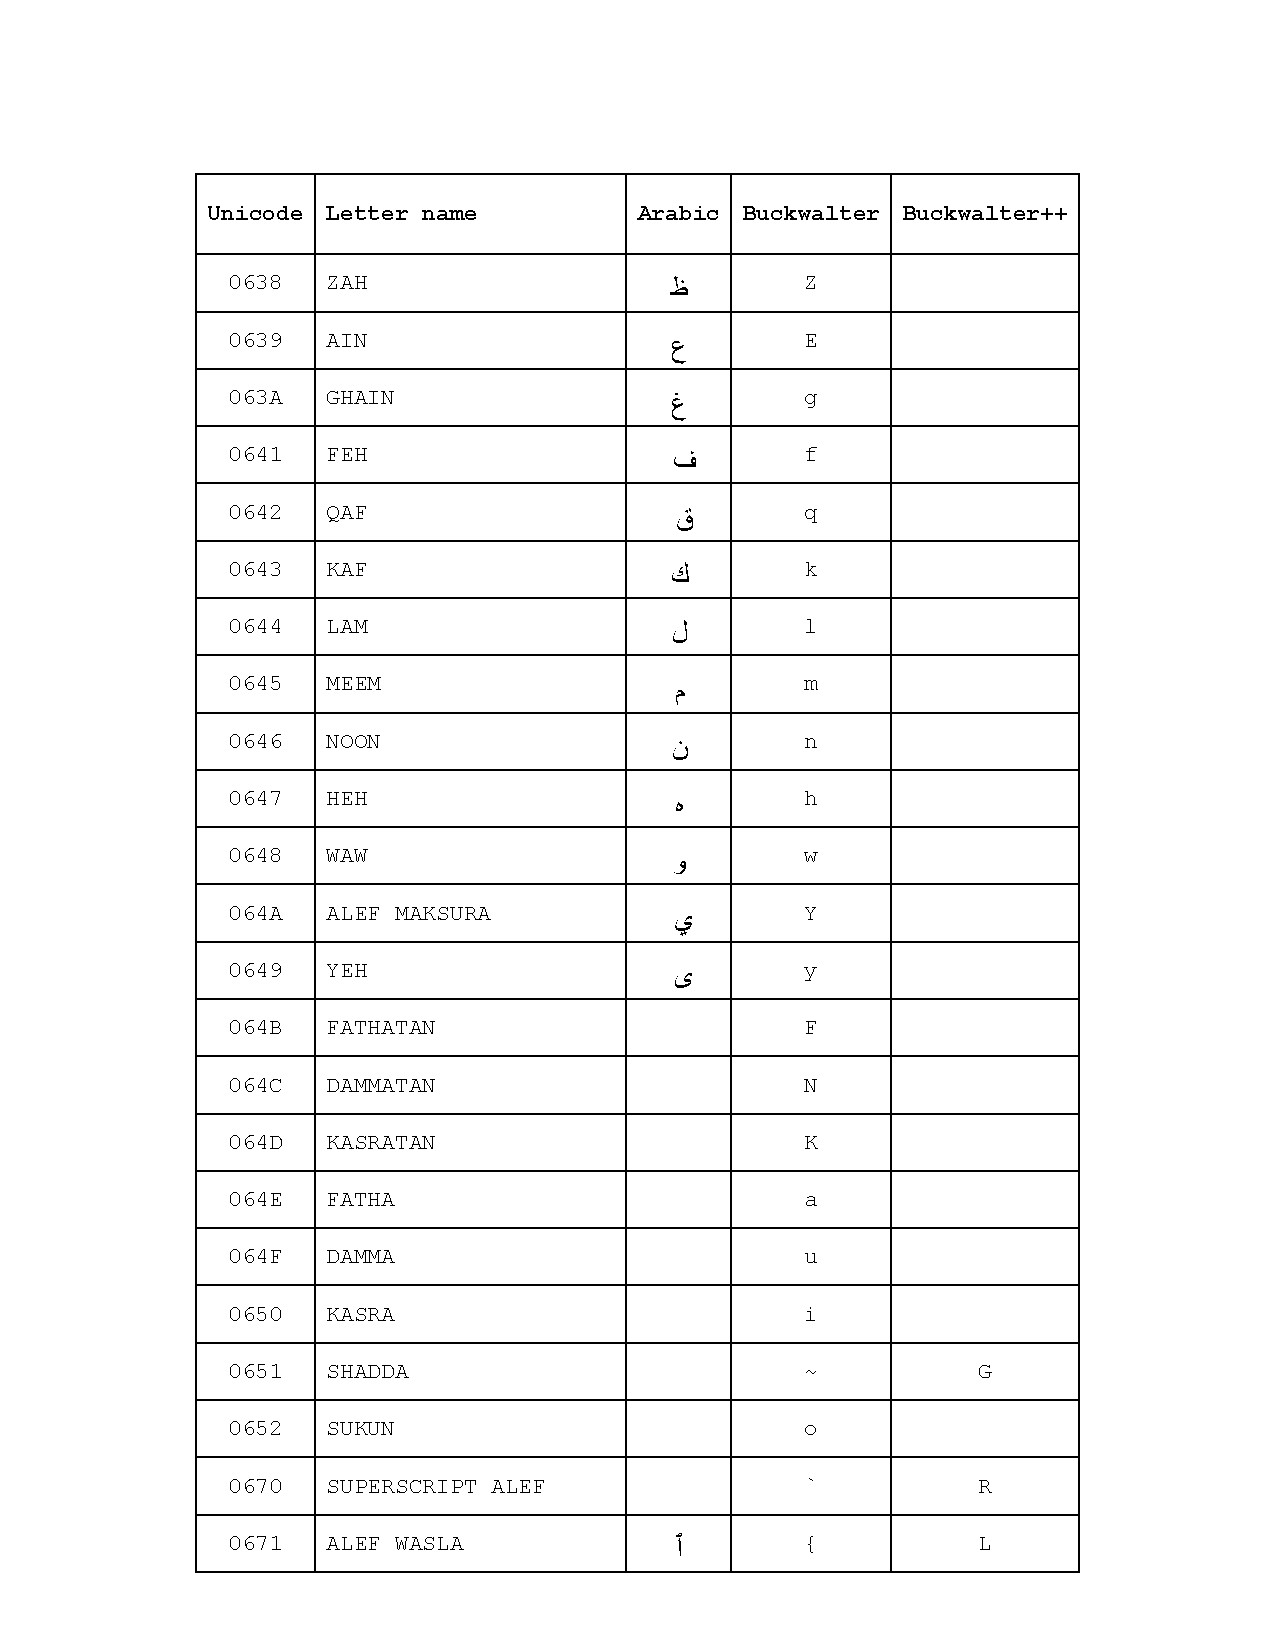
\includegraphics[height=23.5cm]{resources/img/buckwalter2.pdf}
\caption{Buckwalter++ transliteration table, second half\label{buckwalter2}}
\end{center}
\end{figure}

\begin{figure}[!ht]
\begin{center}
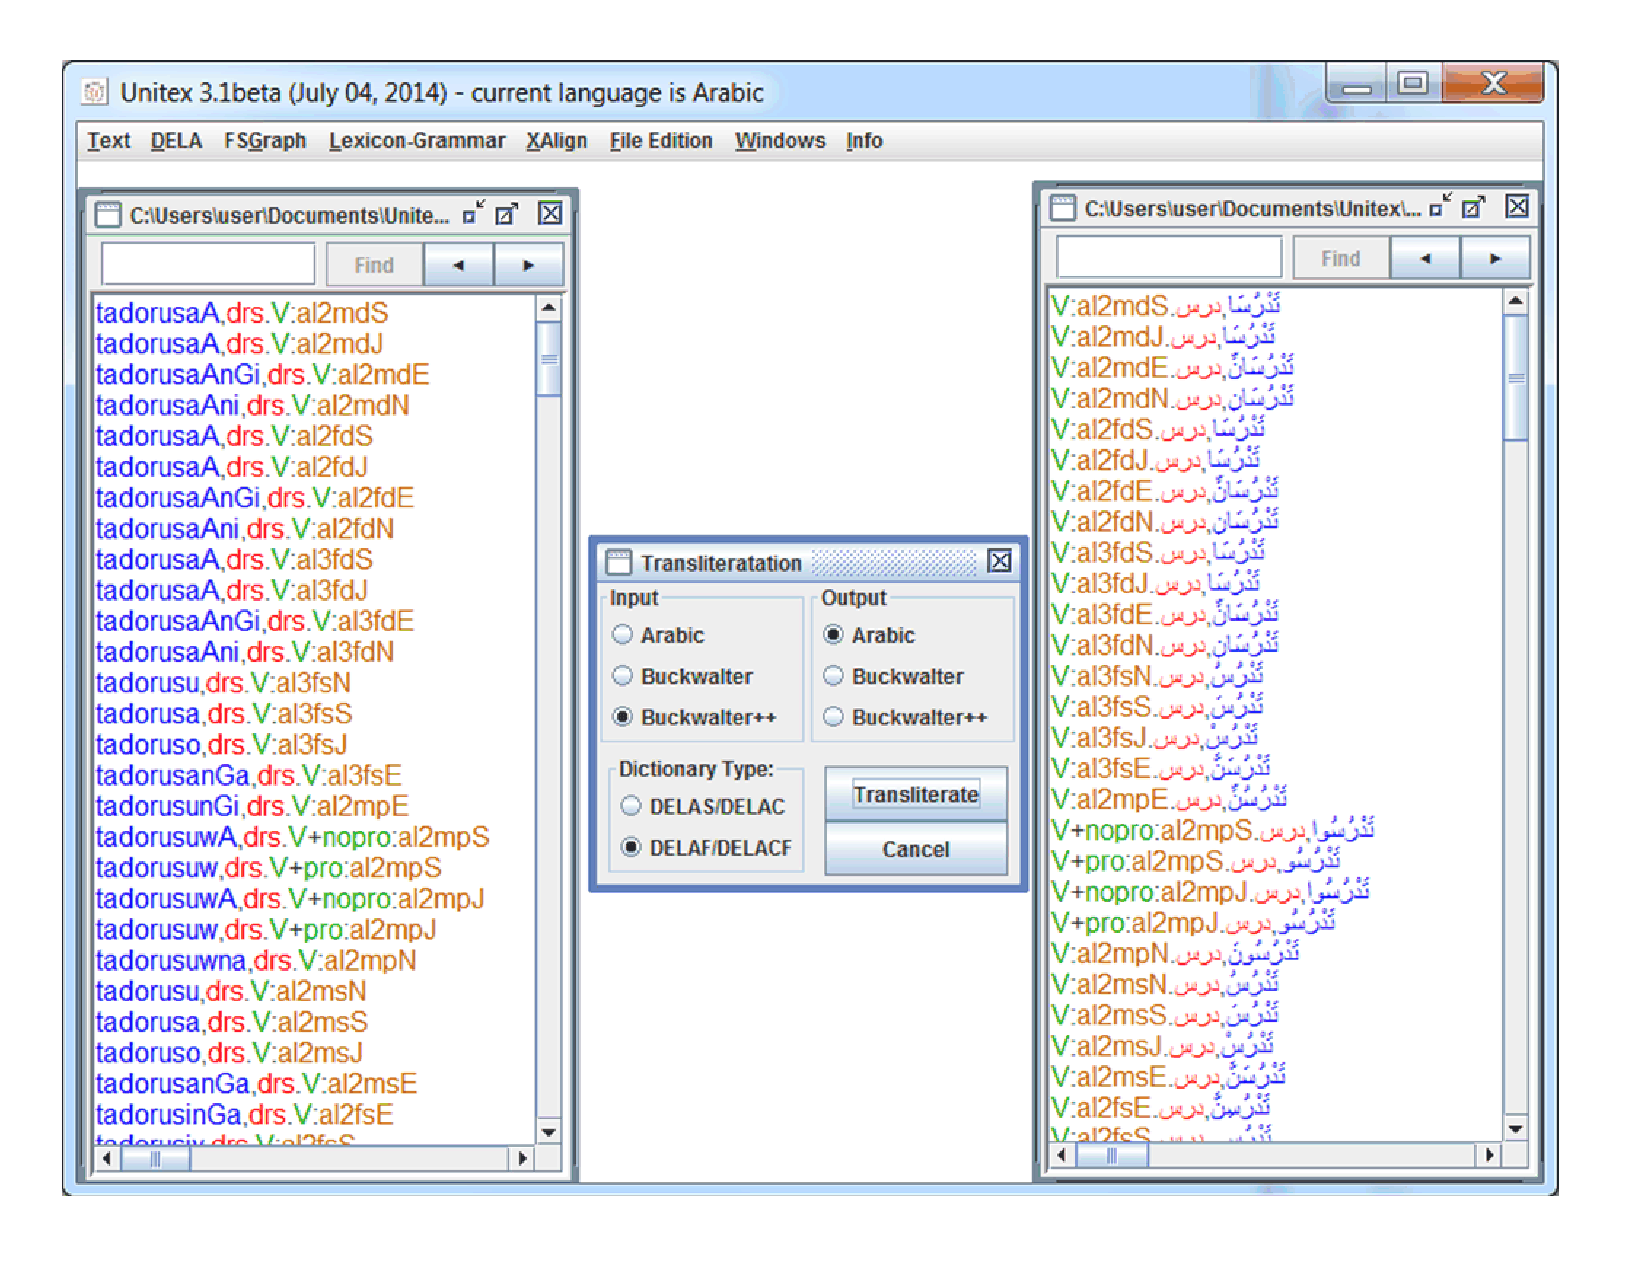
\includegraphics[width=15cm]{resources/img/Arabic-transliteration.pdf}
\caption{Transliteration of a DELAF
dictionary from Buckwalter++ (left) to the Arabic script (right)\label{Arabic-transliteration}}
\end{center}
\end{figure}



\section{Compression}
\index{Dictionaries!compression}

Unitex applies compressed dictionaries to the text. The compression reduces the
size of the dictionaries and speeds up the lookup. This operation is done by the
\verb+Compress+ program. \index{\verbc{Compress}}\index{External
programs!\verbc{Compress}}This program takes a dictionary in text form 
as input (for example \verb+my_dico.dic+) and produces two files:

\index{File!\verbc{.dic}}
\begin{itemize}
  \item \verb+my_dico.bin+ contains the minimal automaton of the inflected forms of the dictionaries;
  \index{File!\verbc{.bin}}
  \item \verb+my_dico.inf+ contains the codes extracted from the original dictionary.\index{File!\verbc{.inf}}
\end{itemize}

\index{Automaton!minimal}
\noindent The minimal automaton in the \verb+my_dico.bin+ file is a
representation of inflected forms in which all common prefixes and suffixes are factorized. For
example, the minimal automaton of the words \verb+me+, \verb+te+, \verb+se+,
\verb+ma+, \verb+ta+ et \verb+sa+ can be represented by the graph shown in
Figure~\ref{fig-example-minimal-automaton}.
\begin{figure}[!ht]
\begin{center}
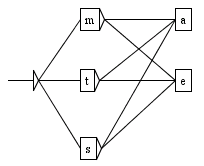
\includegraphics[width=5cm]{resources/img/fig3-10.png}
\caption{Representation of a minimal
automaton\label{fig-example-minimal-automaton}}
\end{center}
\end{figure}

\noindent To compress a dictionary, open it and click on "Compress into FST" in
the "DELA" menu. The compression is independent from the language and from the content of
the dictionary. The messages produced by the program are displayed in a window
that is not closed automatically. You can see the size of the resulting
\verb+.bin+ file, the number of lines read and the number of inflectional codes
created. Figure~\ref{fig-compression-result} shows the result of
the compression of a dictionary of simple words. \bigskip
\begin{figure}[!ht]
\begin{center}
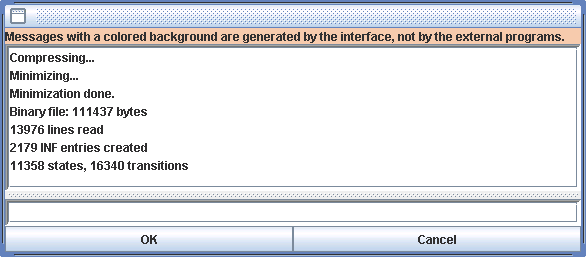
\includegraphics[width=14cm]{resources/img/fig3-11.png}
\caption{Results of a compression\label{fig-compression-result}}
\end{center}
\end{figure}

\bigskip
\noindent The resulting files are compressed to about 95\% for dictionaries containing
simple words and 50\% for those with compound words.

\bigskip
\noindent When the Semitic mode (\ref{subsection-semitic-inflection}) has been heavily used
to inflect a dictionary, a specific variant of the compression algorithm may reduce the size of the
resulting \verb+.bin+ and \verb+.inf+ files. In order to use it, either declare the language as
being a Semitic one in the global preferences by checking the ''Semitic language'' option in
''Preferences > Language and Presentation'', or use the Compress program in command line with the
\verb+--semitic+ option.


\section{Applying dictionaries}
\label{section-applying-dictionaries}
\index{Dictionaries!applying}
Dictionaries can be applied (1) after pre-processing or (2) by explicitly 
clicking on "Apply Lexical Resources" in the  "Text" menu (see
section~\ref{text-applying-dictionaries}).

\bigskip
\noindent Unitex can manipulate compressed dictionaries (\verb+.bin+) and
dictionary graphs (\verb+.fst2+). We will now describe  the rules for applying dictionaries
in detail. Dictionary graphs will be described in
section~\ref{section-dictionary-graphs}.

\subsection{Priorities}
\label{section-dictionary-priorities}
\index{Dictionaries!priority}\index{Priority!of dictionaries}
The priority rule says that  if a word in a text is found in a dictionary, this
word will not be taken into account by dictionaries with lower priority.

\bigskip
\noindent This allows for eliminating a part of ambiguity when applying
dictionaries. For example, the French word \textit{par} has a nominal interpretation in the golf
domain. If you don't want to use this meaning, it is sufficient to create a
filter dictionary containing only the entry \verb$par,.PREP$ and to apply this
with highest priority. This way, even if simple word dictionaries contain 
different entries, they will be ignored given the priority rule.
\index{Dictionaries!filters}

\bigskip
\noindent There are three priority levels. The dictionaries whose names without
extension end with~\verb+-+
\index{\verbc{-}}\index{\verbc{+}}
have the highest priority; those that end with~\verb-+- have the lowest one.
All other dictionaries are applied with medium priority. The order in which
dictionaries with the same priority are applied does not matter.
On the command line, the command:

\bigskip
\noindent
\verb$Dico ex.snt alph.txt ctr+.bin cities-.bin rivers.bin regions-.bin$

\bigskip \noindent will apply the dictionaries in the following order
(\verb+ex.snt+ is the text to which the dictionaries are applied, and 
\verb+alph.txt+ is the alphabet file used):

\bigskip
\begin{enumerate}
  \item \verb$cities-.bin$
  \item \verb$regions-.bin$
  \item \verb$rivers.bin$
  \item \verb$ctr+.bin$
\end{enumerate}

\subsection{Application rules for dictionaries}
\label{section-transducer-application-rules}

Besides the priority rule, the application of dictionaries respects  upper  case
letters and spaces. The upper case rule is as follows:
\index{Rules!upper case and lower case letters}

\begin{itemize}
  \item if there is an upper case letter in the dictionary, then an upper case
  letter has to be in the text;
  
  \item if a lower case letter is in the dictionary, there can be either an upper
  or lower case letter in the text.
\end{itemize}

\bigskip
\noindent Thus, the entry \verb$peter,.N:fs$ will match the words \verb+peter+,
\verb+Peter+ et \verb+PETER+, while

% do not remove this line jump
\noindent \verb$Peter,.N+firstName$ only 
recognizes \verb+Peter+ and \verb+PETER+. Lower and upper case
letters are defined in the alphabet file passed to the \verb+Dico+ program\index{\verbc{Dico}}
\index{External programs!\verbc{Dico}}\index{File!\verbc{Alphabet.txt}}\index{File!alphabet}\index{Alphabet}
as a parameter.

\index{Rules!white space}
\bigskip
\noindent Respecting white space is a very simple rule: For each sequence in the text to be
recognized by a dictionary entry, it has to have exactly the same number of
spaces. For example, if the dictionary contains \verb+aujourd'hui,.ADV+, the
sequence \verb+Aujourd' hui+ will not be recognized because of the space that
follows the apostrophe.


\subsection{Dictionary graphs}
\label{section-dictionary-graphs}\index{Dictionary graphs}
The \verb+Dico+\index{\verbc{Dico}}\index{External programs!\verbc{Dico}} program
can also apply dictionary graphs. Dictionary graphs,
by default,\footnote{Morphological dictionary-graphs are an exception (section
\ref{section-morphological-dictionary-graphs}) .}
conform to the following rule: if applied by \verb+Locate+\index{\verbc{Locate}}\index{External
programs!\verbc{Locate}} in MERGE\index{MERGE} mode,
they must produce output sequences that are valid DELAF lines.\index{DELAF}\index{Dictionaries!DELAF}
When they are applied to a text, they attach the DELAF lexical labels to the sequences.

\begin{figure}[!p]
\begin{center}
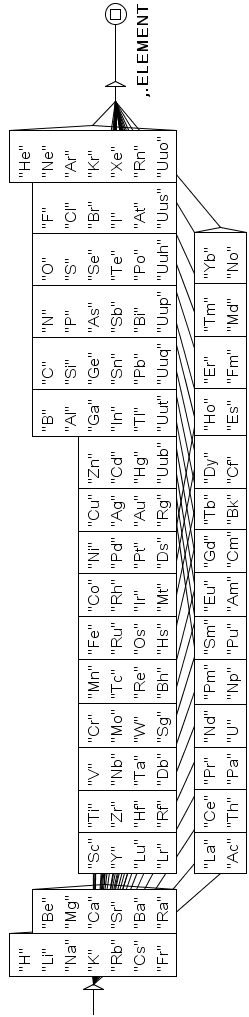
\includegraphics[height=24cm]{resources/img/fig3-12.png}
\caption{Dictionary graph of chemical elements\label{elements}}
\end{center}
\end{figure}

\bigskip
\noindent Figure \ref{elements} shows a graph that recognizes chemical
elements. We can observe a first advantage of graphs over usual dictionaries: we can force case
with double quotes. Thus, this graph will
correctly match \verb+Fe+ but not \verb+FE+, while this restriction cannot be specified in a
normal DELAF.

\bigskip
\noindent Another advantage of dictionary graphs is that they can use results
given by previous dictionaries. Thus, it is possible to apply the standard dictionary, and then tag as proper
names all the unknown words that begin with an uppercase letter, thanks to
graph \verb$NPr+$ shown in figure~\ref{graph-NPr}. The \verb$+$ in the graph
name gives to it a low priority, so that it will be applied after the standard
dictionary. This graph works with words that are still unknown after the
application of the standard dictionary. Square brackets stand for a context definition.
For more information about contexts,\index{Contexts!zone in a graph} see section
\ref{section-contexts}.

\begin{figure}[!ht]
\begin{center}
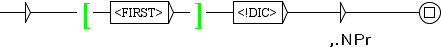
\includegraphics[width=10.5cm]{resources/img/fig3-13.png}
\caption{Dictionary graph that tags unknown words beginning with an uppercase letter as proper names\label{graph-NPr}}
\end{center}
\end{figure}

\noindent Since dictionary graphs are applied using the engine of \verb+Locate+,
they have exactly the same properties than syntactic graphs. So,
you can use morphological filters (section~\ref{section-filters})
and/or the morphological mode (section~\ref{section-morphological-mode}).
\index{Morphological filters}\index{Morphological mode}For instance, the
graph shown on Figure \ref{graph-CR} uses morphological filters to recognize
roman numerals. Note that it also uses contexts in order to avoid recognizing 
uppercase letters in some contexts.

\begin{figure}[!p]
\begin{center}
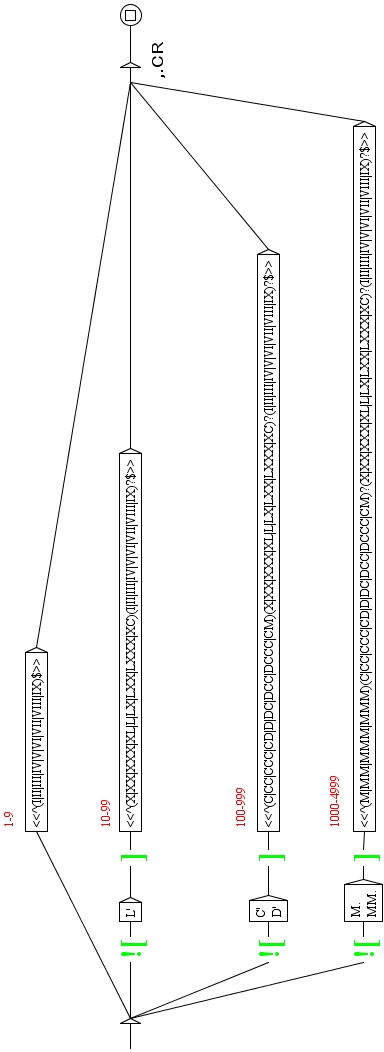
\includegraphics[height=24cm]{resources/img/fig3-14.png}
\caption{Dictionary graph of roman numerals\label{graph-CR}}
\end{center}
\end{figure}

\bigskip
\noindent By default, dictionary graphs are applied in MERGE mode. If you want
to apply them in REPLACE mode, you must suffix graph names with \verb+-r+. This can
be combined with the \verb-+- and \verb+-+ priority marks:

\bigskip
\verb?bagpipe-r.fst2  McAdam-r-.fst2  phtirius-r+.fst2?

\subsubsection{Exporting produced entries as a morphological-mode dictionary}
\index{Morphological-mode dictionaries}
Dictionary entries produced by dictionary graphs are looked up 
by the \verb+Locate+ program when it comes across lexical masks involving dictionary lookup.

\bigskip
\noindent However, this functionality is restricted when the lexical mask is
in morphological mode (section~\ref{section-morphological-mode}).
Dictionary graphs cannot be declared as being morphological-mode 
dictionaries in the usual way (section~\ref{morph-mode-dic}), because they are not \verb+.bin+ files.
When in morphological mode, lexical masks involving dictionary lookup do not trigger lookup of dictionary graphs.
To compensate for this, there are several solutions.
\begin{itemize}
\item Consider invoking the dictionary graph from the part of the graph which is in morphological mode.
\item Unitex internally generates a dictionary of the forms recognized in the text by a dictionary graph.
If the name of the dictionary graph contains the \verb+b+ switch (see Naming conventions below),
Unitex includes this internal dictionary among morphological-mode dictionaries, so that it is looked up
when the \verb+Locate+ program comes across lexical masks in morphological mode. But this
solution works only for forms recognised in the text by the dictionary graph during initial application
 of dictionaries (section~\ref{section-applying-dictionaries}), and not for forms that appear in the text only as token parts.
\end{itemize}
If you add \verb+z+ instead of \verb+b+, then the dictionary internally generated for the text
is compressed immediately, and  can be looked up when other dictionary graphs are applied later.
 
\subsubsection{Naming conventions}
The whole naming scheme for dictionary graphs is as follows:

\verb$name(-XYZ)([-+]).fst2$

\noindent where:
\begin{itemize}
\item \verb+X+ is in \verb+[rRmM]+: \verb+r+ means REPLACE mode; \verb+M+ means MERGE mode (default);
\item \verb+Y+ is in \verb+[bBzZ]+: option that rules the production of a morphological-mode dictionary (see above Exporting produced entries as a morphological-mode dictionary);
\item \verb+Z+ is in \verb+[aAlLsS]+: \verb+a+ means that the graph will be applied in "All matches" mode; \verb+l+ means 
      "Longest matches" mode (default); \verb+s+ means "Shortest matches" mode.
\end{itemize}



\subsection{Morphological dictionary-graphs}
\label{section-morphological-dictionary-graphs}\index{Morphological dictionary-graphs}
In a dictionary graph, by default, each path must output a lexical entry to be added in the text
dictionaries. In a morphological dictionary-graph, each path must output
a sequence of one or more tags enclosed in braces and conforming to the syntax
of a DELAF line (section~\ref{section-DELAF-entry-syntax}). The output
of such graphs will be used as special input for the construction of the text
automaton. We call them `morphological dictionary-graphs' because their
main utility is to introduce new morphological analyses in the text automaton,
using the morphological mode (see section \ref{section-morphological-mode}).
This functionality is helpful for agglutinative languages like Korean. To allow the use of a
graph as a morphological dictionary-graph, declare it with a slash (/) as the first
character of its output, as in Figure \ref{morphoA}.


\begin{figure}[!ht]
\begin{center}
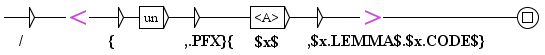
\includegraphics[width=14cm]{resources/img/fig3-14a.png}
\caption{Example of a morphological dictionary-graph\label{morphoA}}
\end{center}
\end{figure}

\noindent The rule is simple: any output of a dictionary graph that begins
with a slash will be added to the file \verb+tags.ind+, \index{\verbc{tags.ind}}
located in the text directory. This file is used by the \verb+Txt2Fst2+ program
in order to add interpretations into the text automaton. The
grammar of Figure \ref{morphoA} matches words made of the prefix
\verb+un+ followed by an adjective. If we apply it as a dictionary
graph, we obtain new paths in the text automaton, as shown on Figure
\ref{morphoB}. Note that when two tags correspond to analyses within the same
token, the link between them is displayed with a dashed line.

\begin{figure}[!ht]
\begin{center}
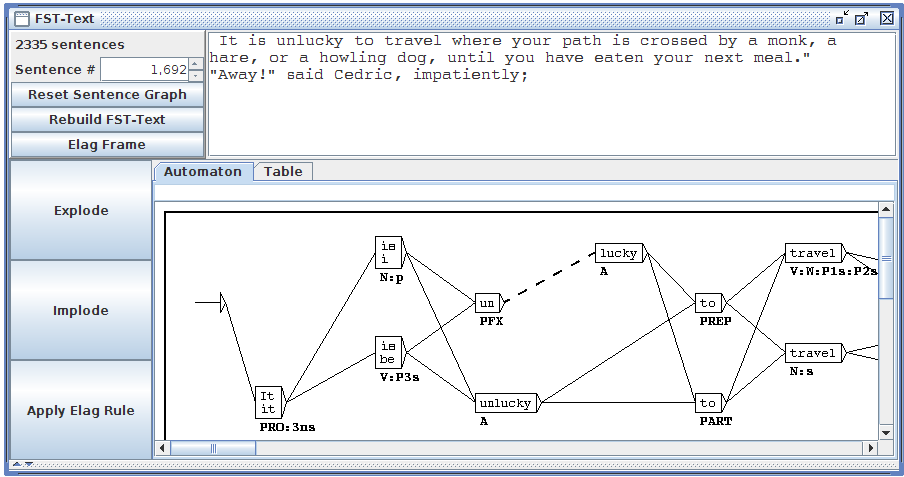
\includegraphics[width=15cm]{resources/img/fig3-14b.png}
\caption{Path added by a morphological dictionary-graph\label{morphoB}}
\end{center}
\end{figure}


\section{Bibliography}


Table~\ref{ref-dicos} gives some references for electronic dictionaries with simple and 
compound words. For more details, see the references page on the Unitex website: \\
\url{http://www-igm.univ-mlv.fr/~unitex}

\begin{table}[!ht]
\begin{center}
\begin{tabular}{|l|c|c|}
\hline
\textbf{Language} & \textbf{Simple words} & \textbf{Compound words} \\
\hline
English & \cite{klarsfeld}, \cite{monceaux-1995} & \cite{delac-anglais},
\cite{these-Savary} \\
\hline
French & \cite{formes-ambigues}, \cite{dicos-francais}, \cite{jacques-1995} & \cite{dicos-francais},
\cite{Gross96},
\cite{max-1993},
\cite{syntaxe-de-ladverbe} \\
\hline
Modern Greek & \cite{modern-greek}, \cite{matthieu-anastasia}, \cite{these-tita} & \cite{tita-2002},
\cite{anastasia-2002} \\
\hline
Italian & \cite{delaf-italien}, \cite{delaf-italien-book} & \cite{composes-italien} \\
\hline
Spanish & \cite{blanco-2000} & \cite{blanco-1997} \\
\hline
Portuguese & \cite{eleuterio1995}, \cite{ranchhod1996b}, \cite{ranchhodd1998},
\cite{muniz2005} & \cite{ranchhod1991}, \cite{ranchhodd1998} \\
\hline
\end{tabular}
\caption{Some bibliographical references for electronic dictionaries\label{ref-dicos}}
\end{center}
\end{table}
